\section{Model Evaluation}

\subsection{Evaluation Metrics}
Multiple metrics are applied to evaluate the model performance on our garbage dataset, including top-k accuracy, confusion matrix, precision, recall and F1-score.

\subsubsection{Top-k Accuracy}
Top-k accuracy is when you measure how often your predicted class falls in the top k values of your softmax distribution\cite{topk}. we use top-1 and top-5 accuracy to measure how well the model predict the whole validation dataset. We draw both the training and validation accuracy curve during the training procedure, which is show in Figure \ref{fig:train_acc1}, Figure \ref{fig:train_acc5}, Figure \ref{fig:val_acc1} and Figure \ref{fig:val_acc5}. The best performance of baseline models on the garbage dataset is concluded in Table \ref{tabel:train_acc} and Table \ref{tabel:val_acc}.

\begin{figure}[ht]
  \begin{minipage}[t]{0.5\linewidth}
    \centering
    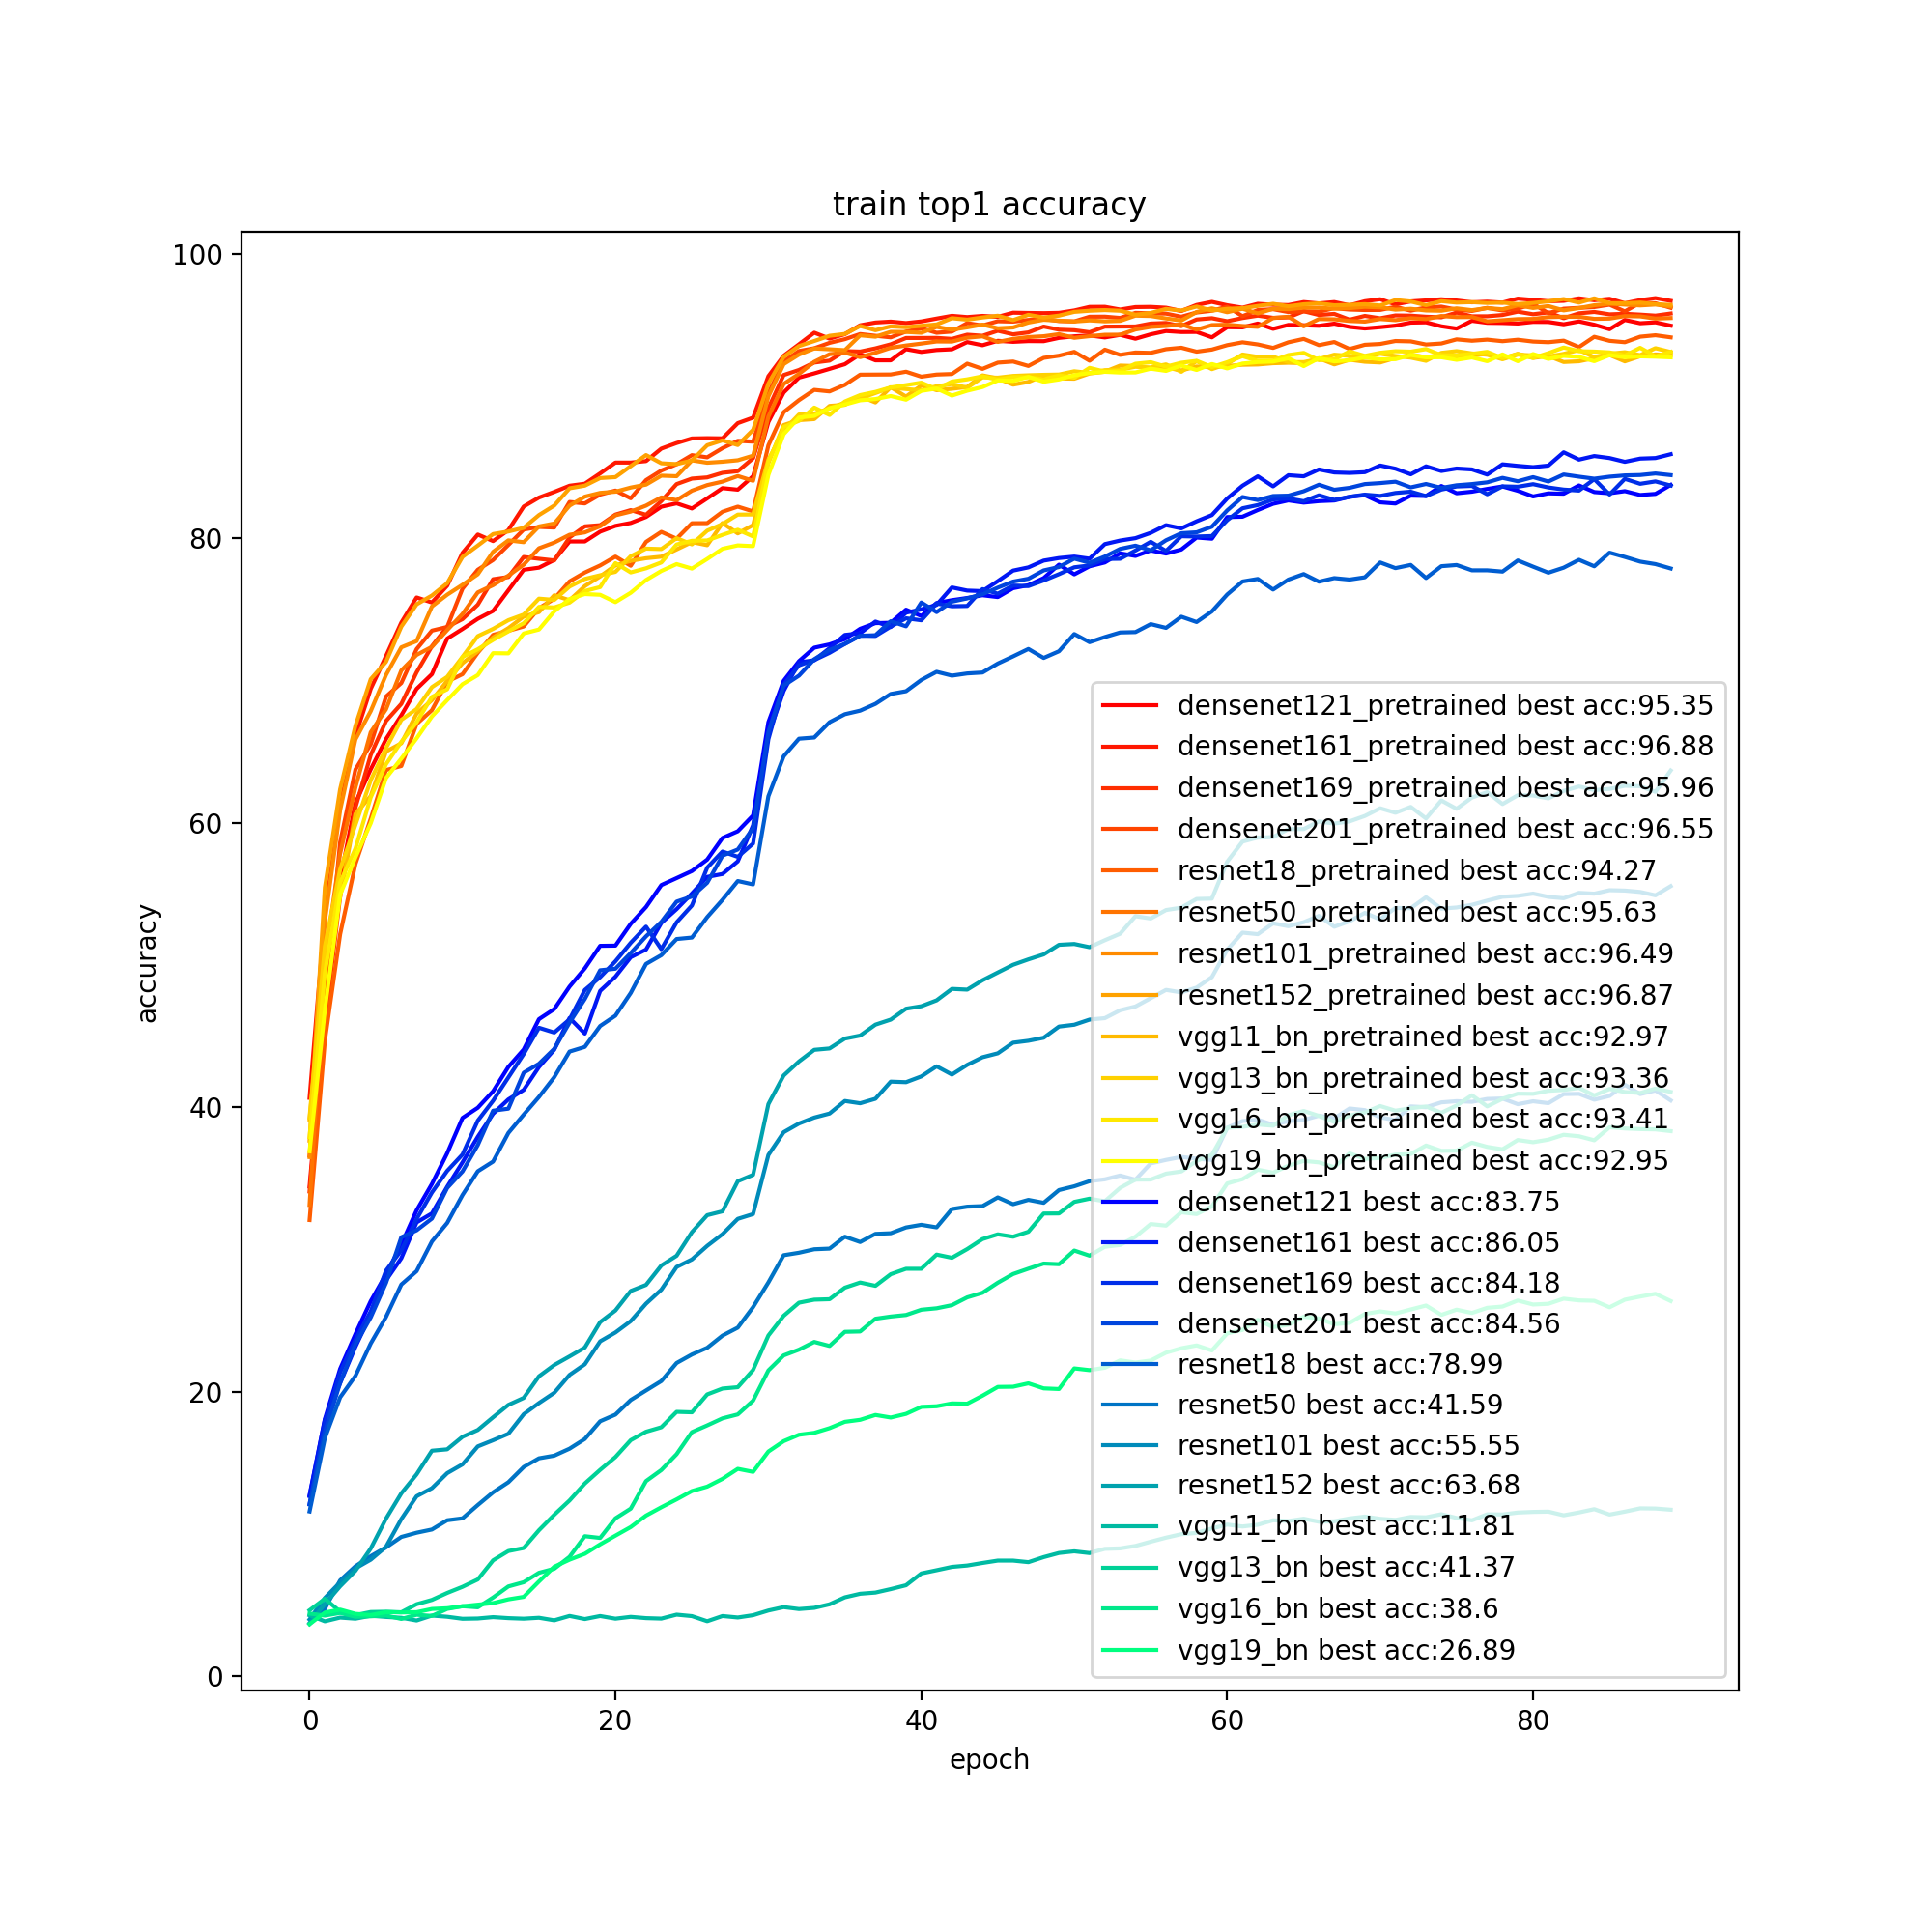
\includegraphics[width=1.1\textwidth]{figs/train_acc1.png}
    \subcaption{Top-1 accuracy}
    \label{fig:train_acc1}
  \end{minipage}\hfill
  \begin{minipage}[t]{0.5\linewidth}
    \centering
    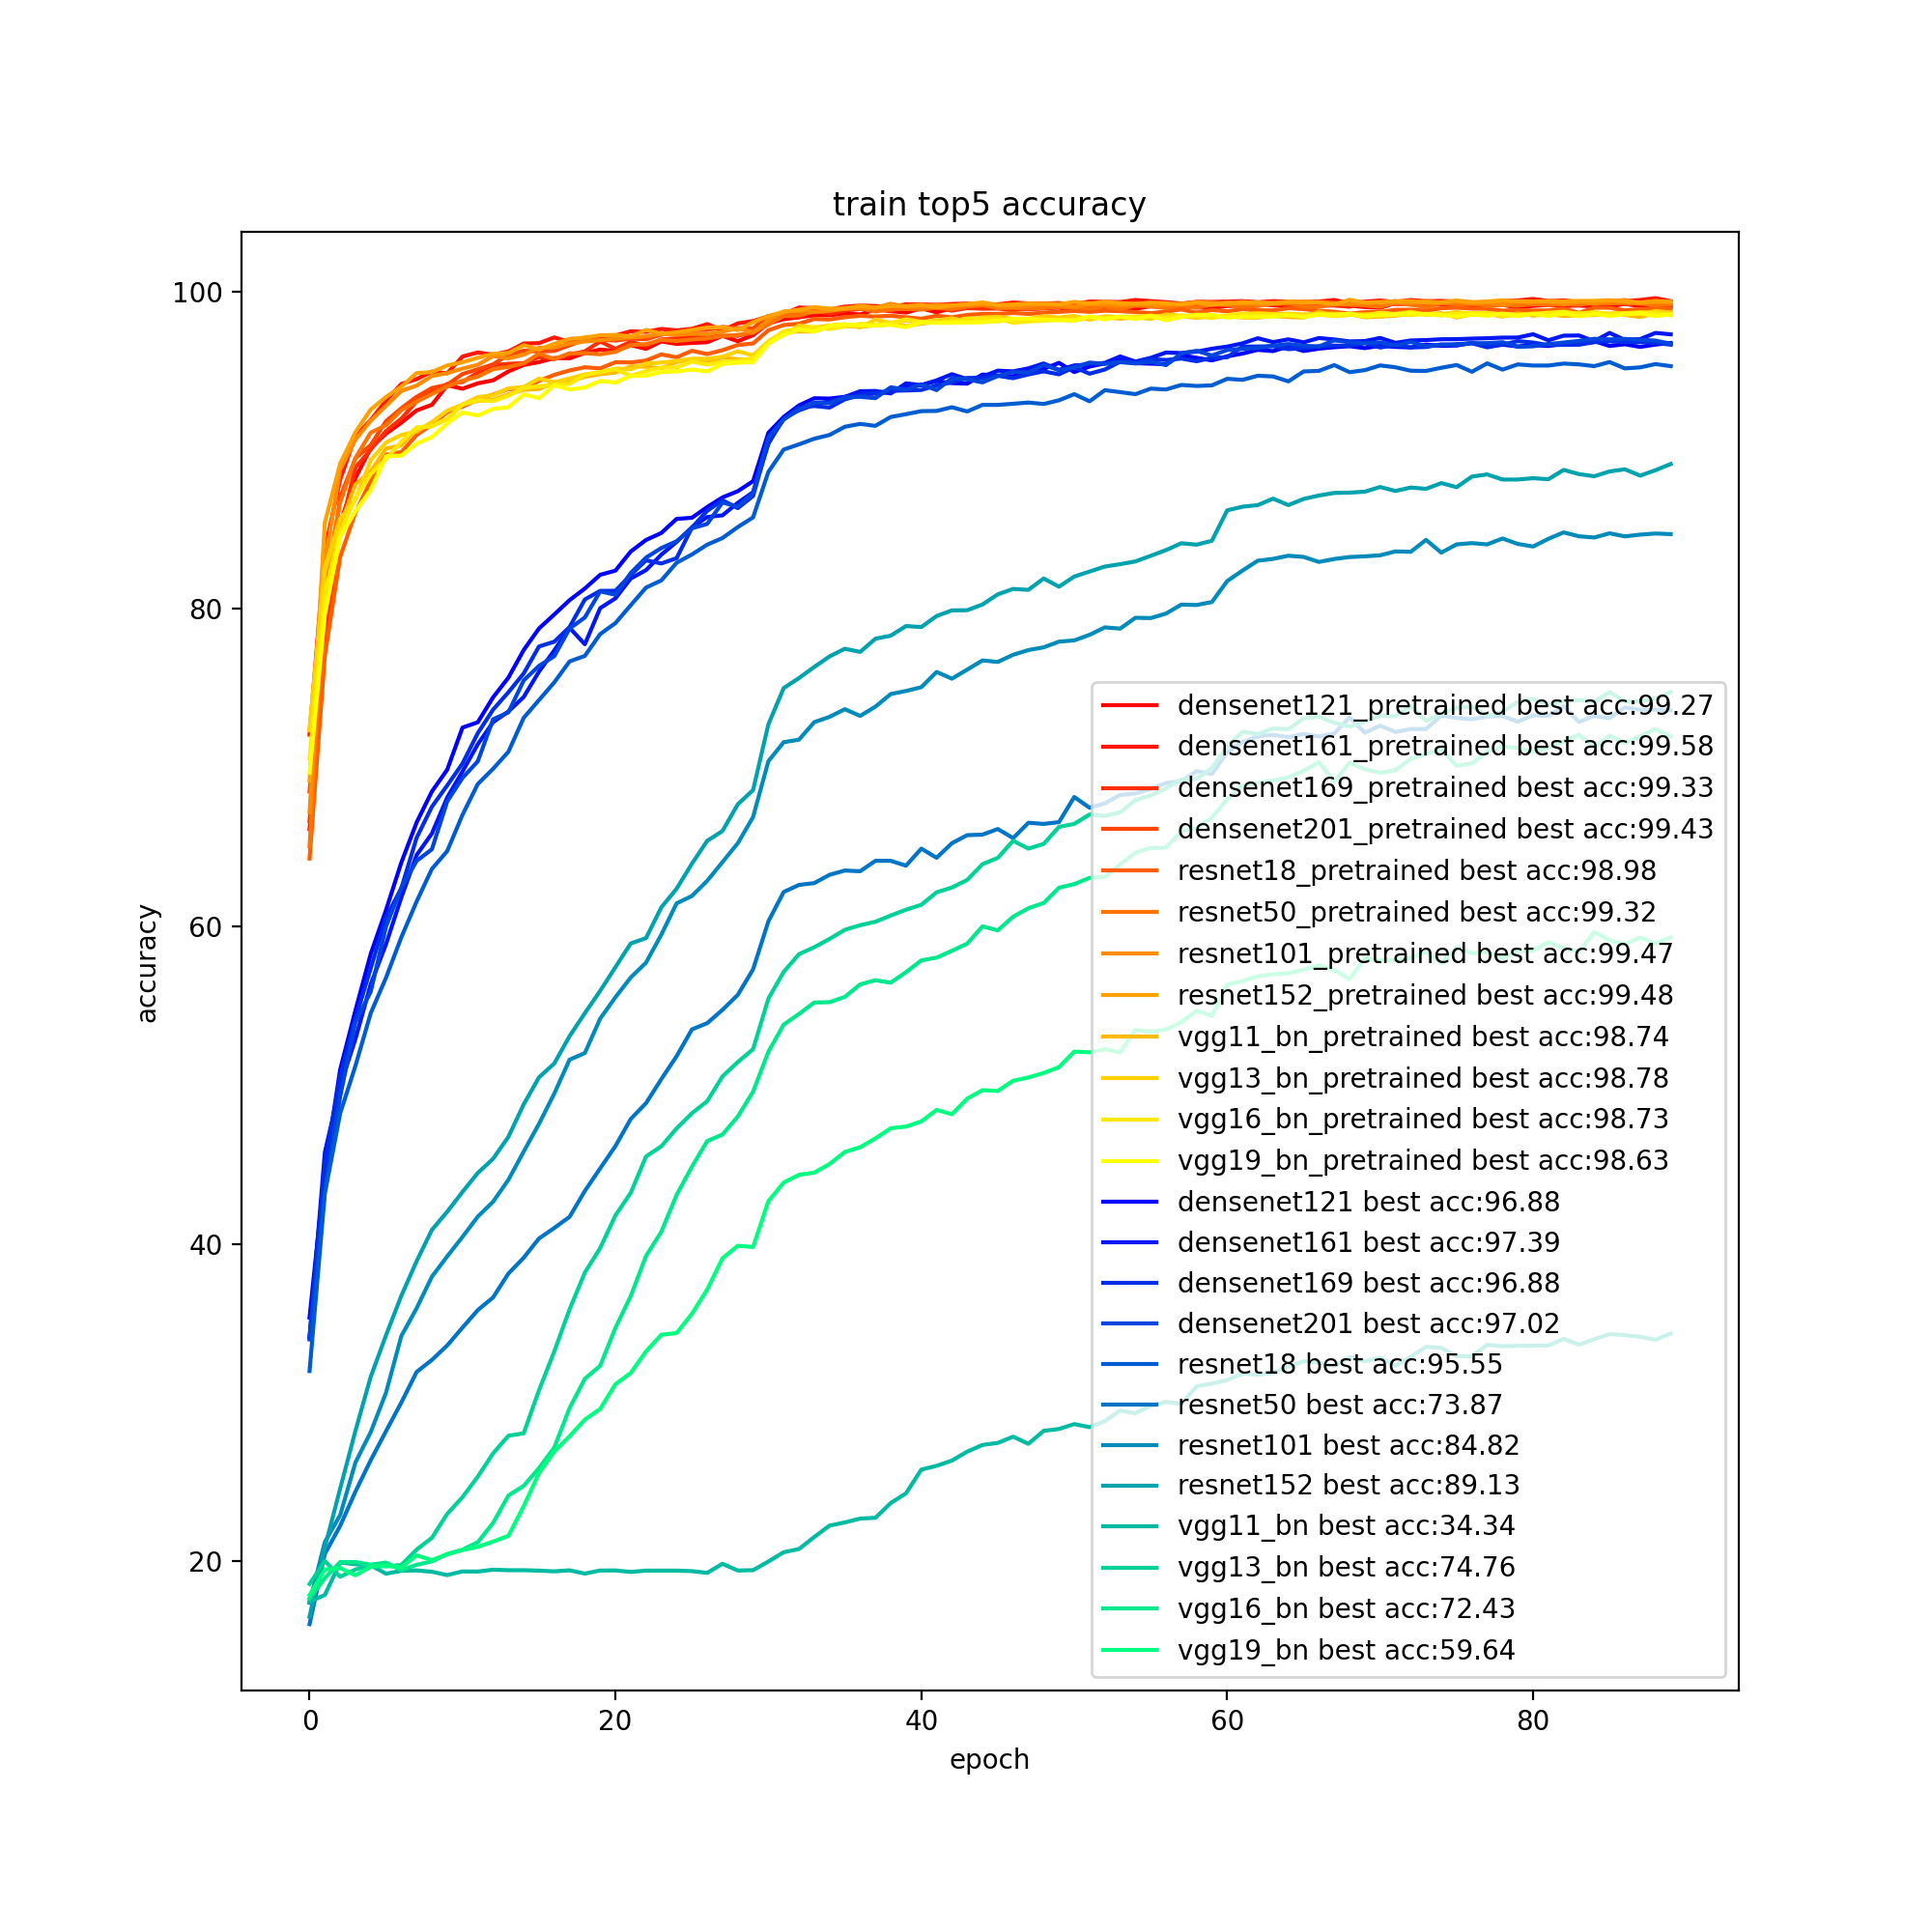
\includegraphics[width=1.1\textwidth]{figs/train_acc5.png}
    \subcaption{Top-5 accuracy}
    \label{fig:train_acc5}
  \end{minipage}
  \caption{Training accuracy of baseline models}
\end{figure}

% \begin{figure}[ht]
%   \centering
%   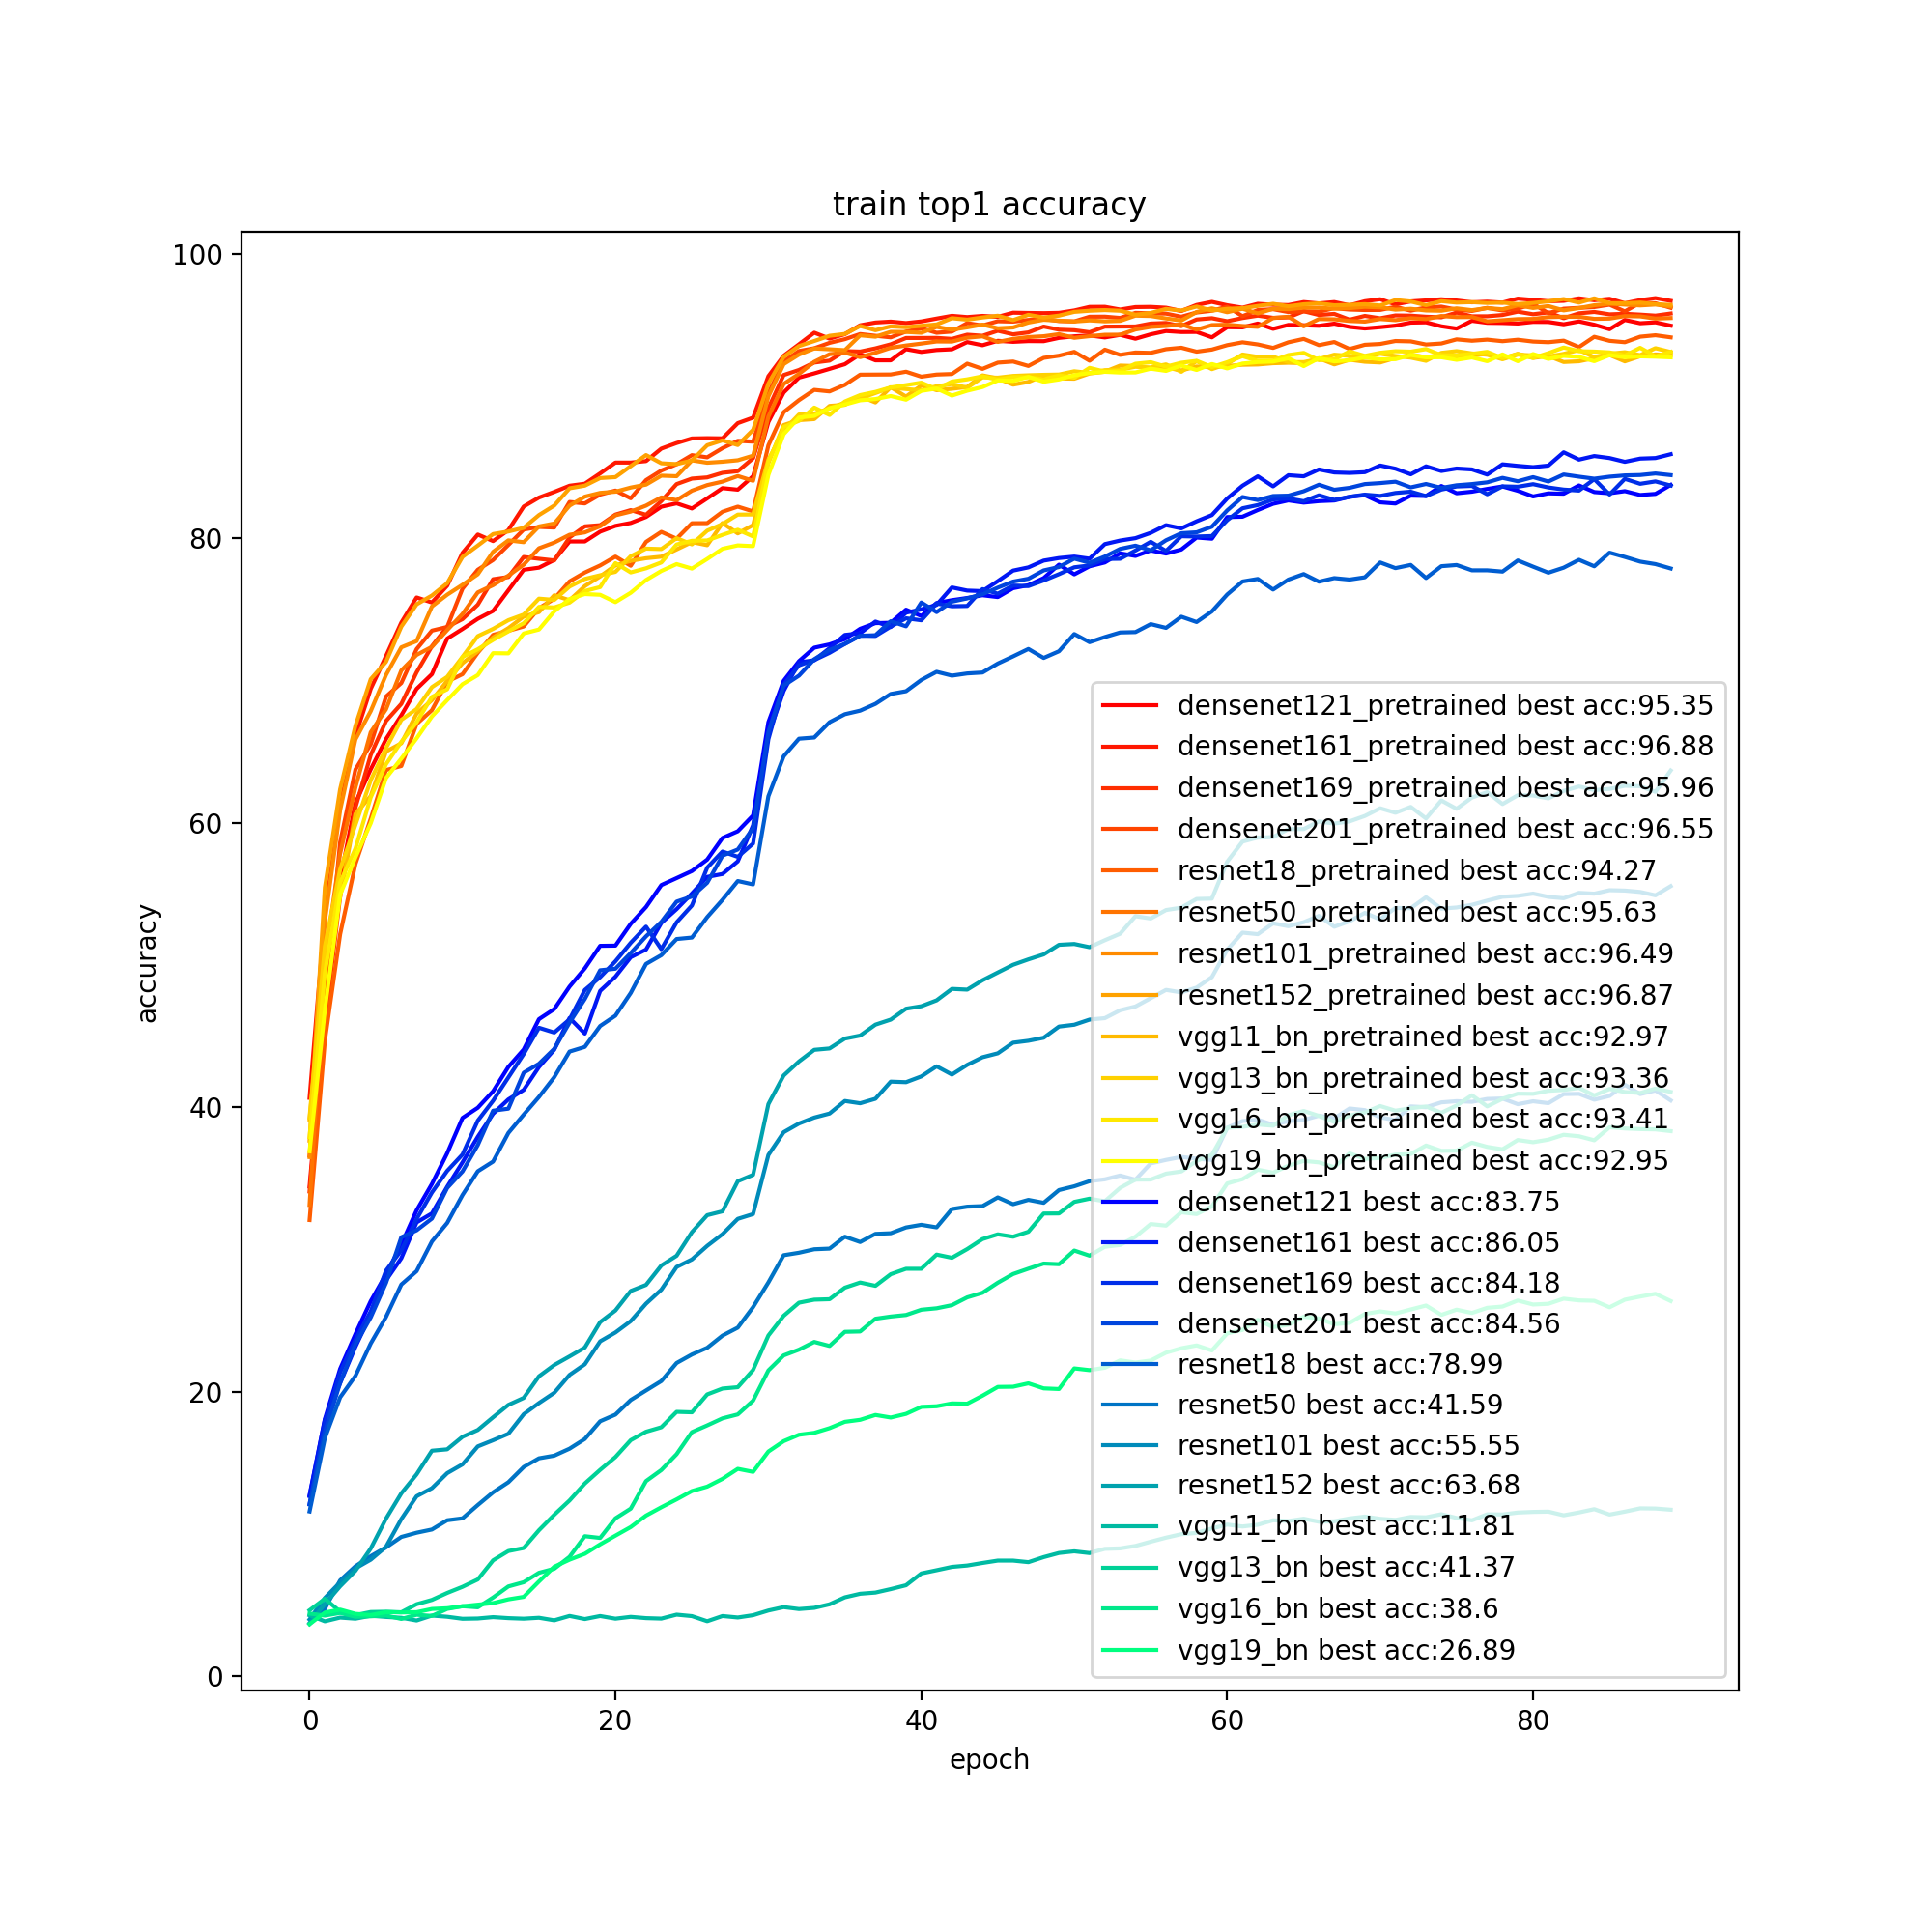
\includegraphics[scale=0.4]{figs/train_acc1.png}
%   \caption{Top-1 Train Accuracy of Baseline Models}
%   \label{fig:train_acc1}
% \end{figure}

% \begin{figure}[ht]
%   \centering
%   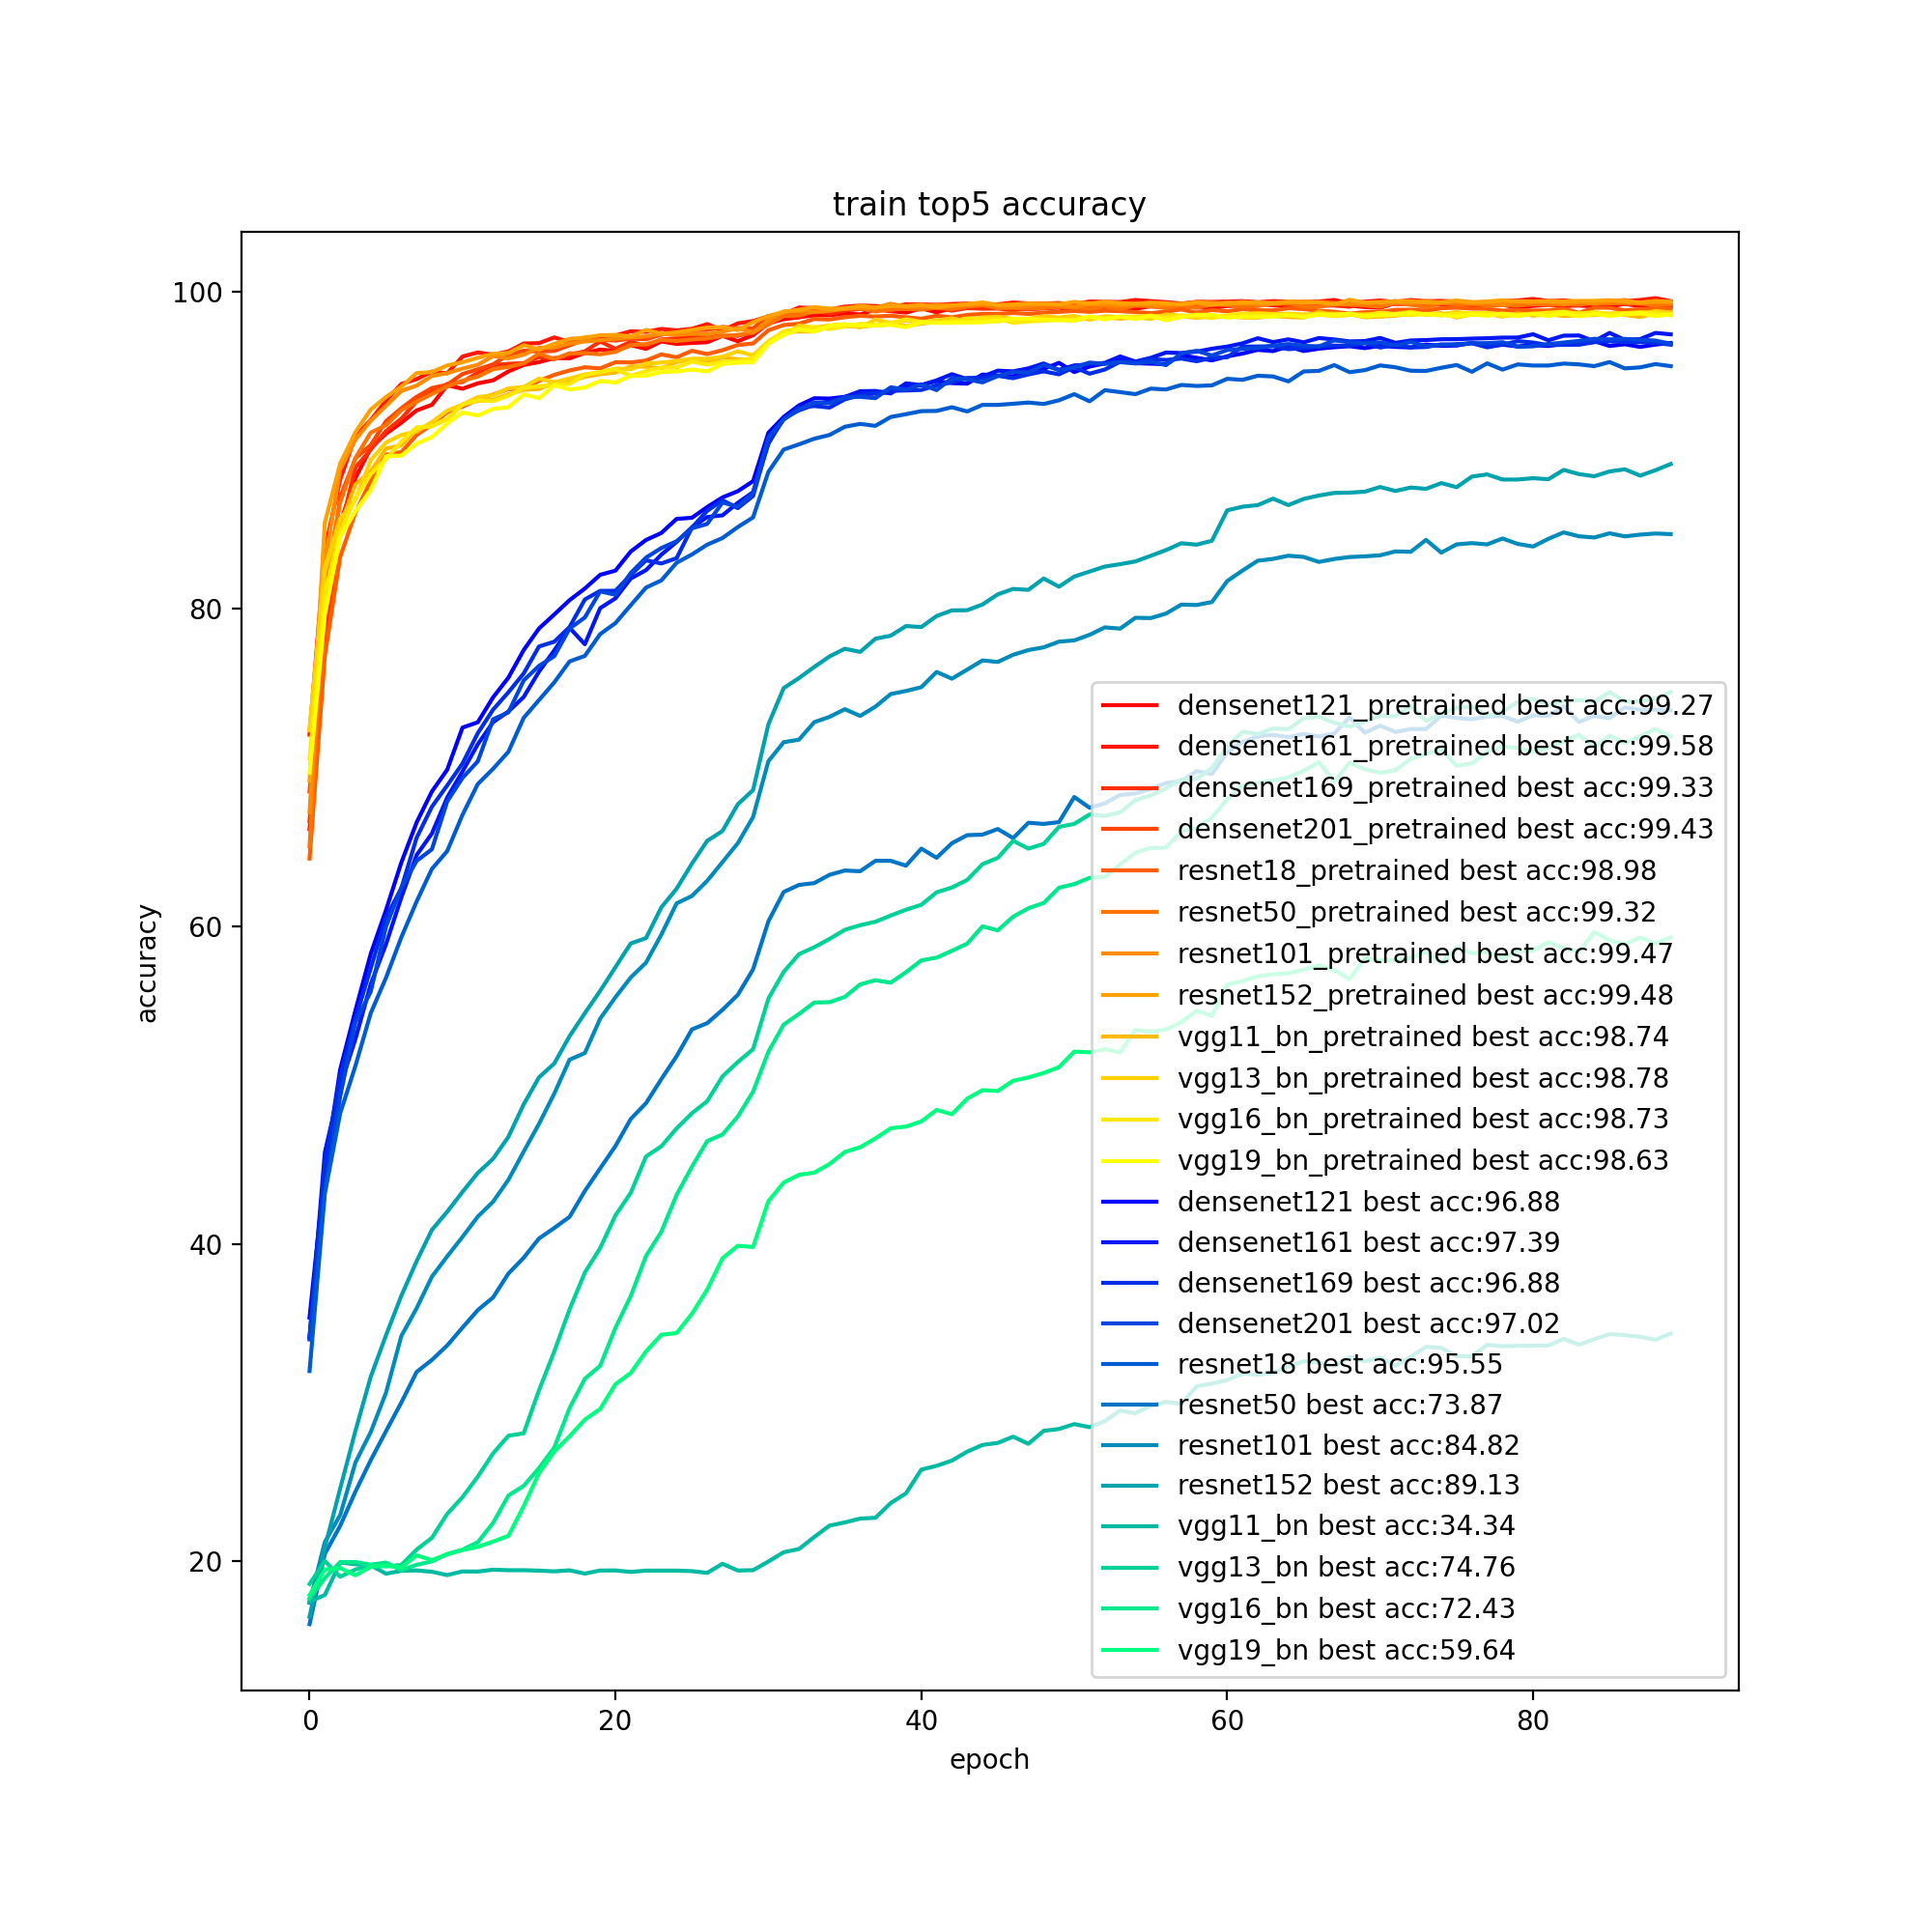
\includegraphics[scale=0.4]{figs/train_acc5.png}
%   \caption{Top-5 Train Accuracy of Baseline Models}
%   \label{fig:train_acc5}
% \end{figure}

\begin{figure}[ht]
  \begin{minipage}[t]{0.5\linewidth}
    \centering
    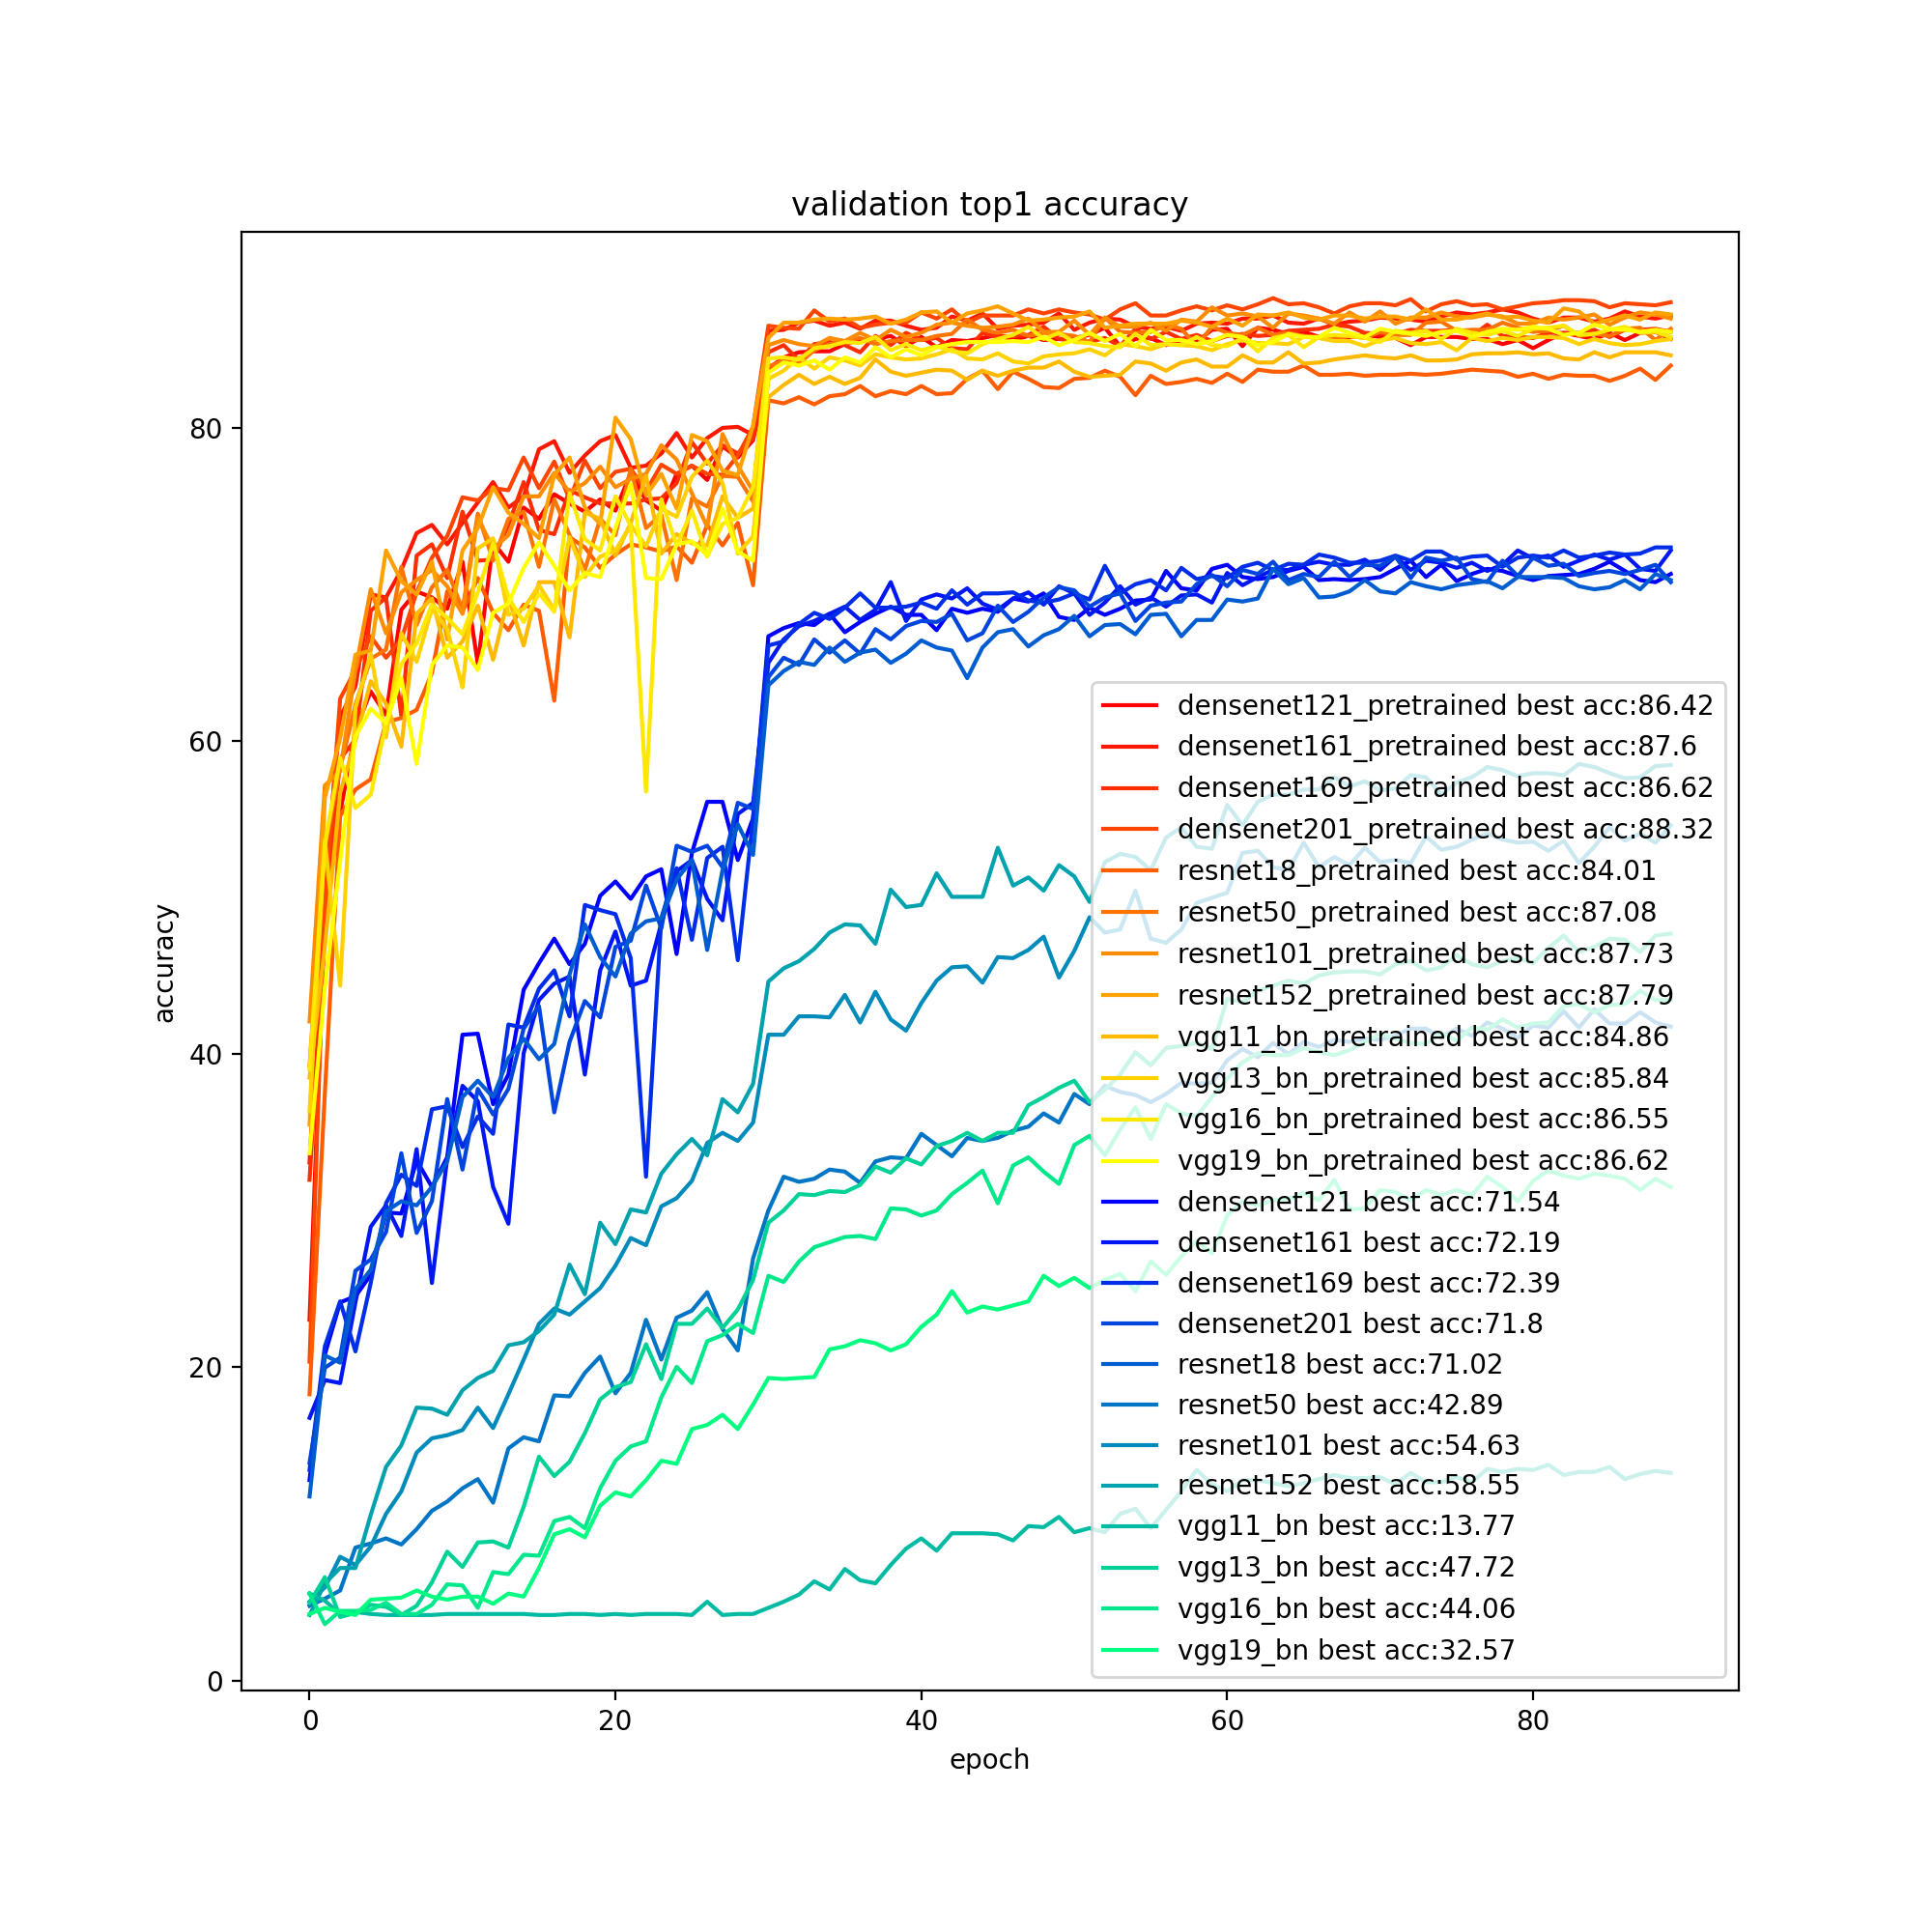
\includegraphics[width=1.1\textwidth]{figs/val_acc1.png}
    \subcaption{Top-1 accuracy}
    \label{fig:val_acc1}
  \end{minipage}\hfill
  \begin{minipage}[t]{0.5\linewidth}
    \centering
    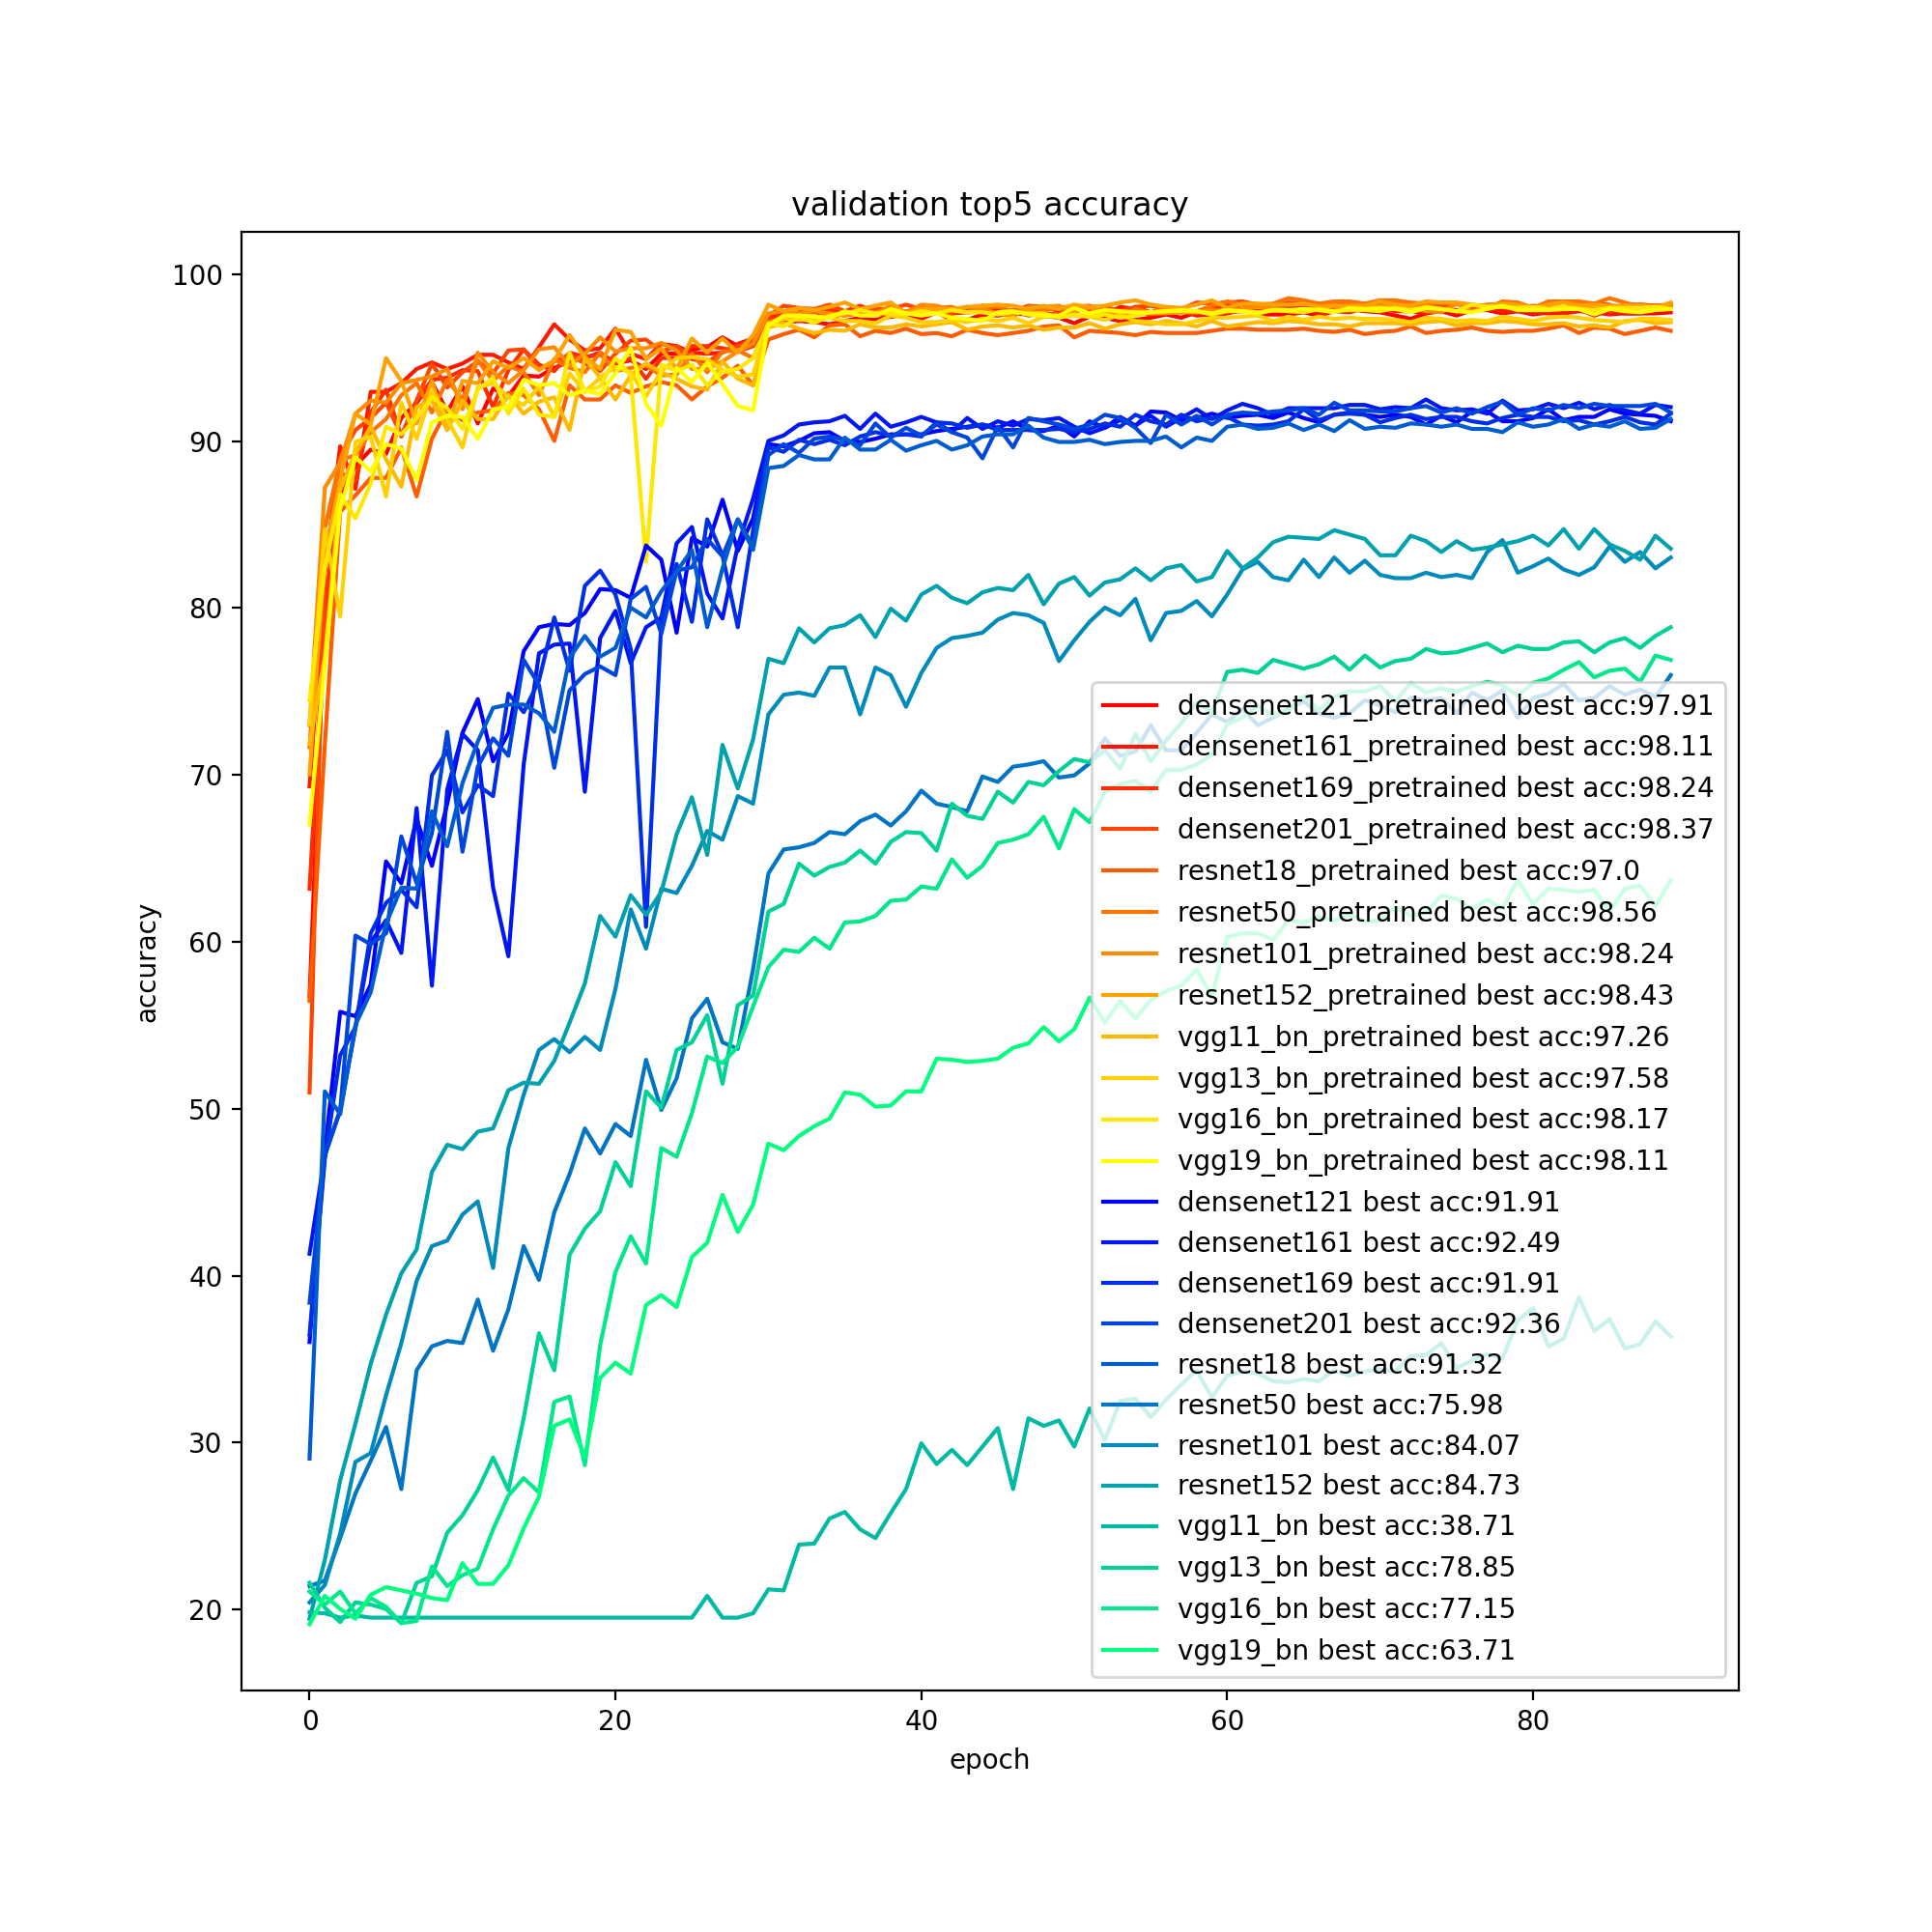
\includegraphics[width=1.1\textwidth]{figs/val_acc5.png}
    \subcaption{Top-5 accuracy}
    \label{fig:val_acc5}
  \end{minipage}
  \caption{Validation accuracy of baseline models}
\end{figure}

% \begin{figure}[ht]
%   \centering
%   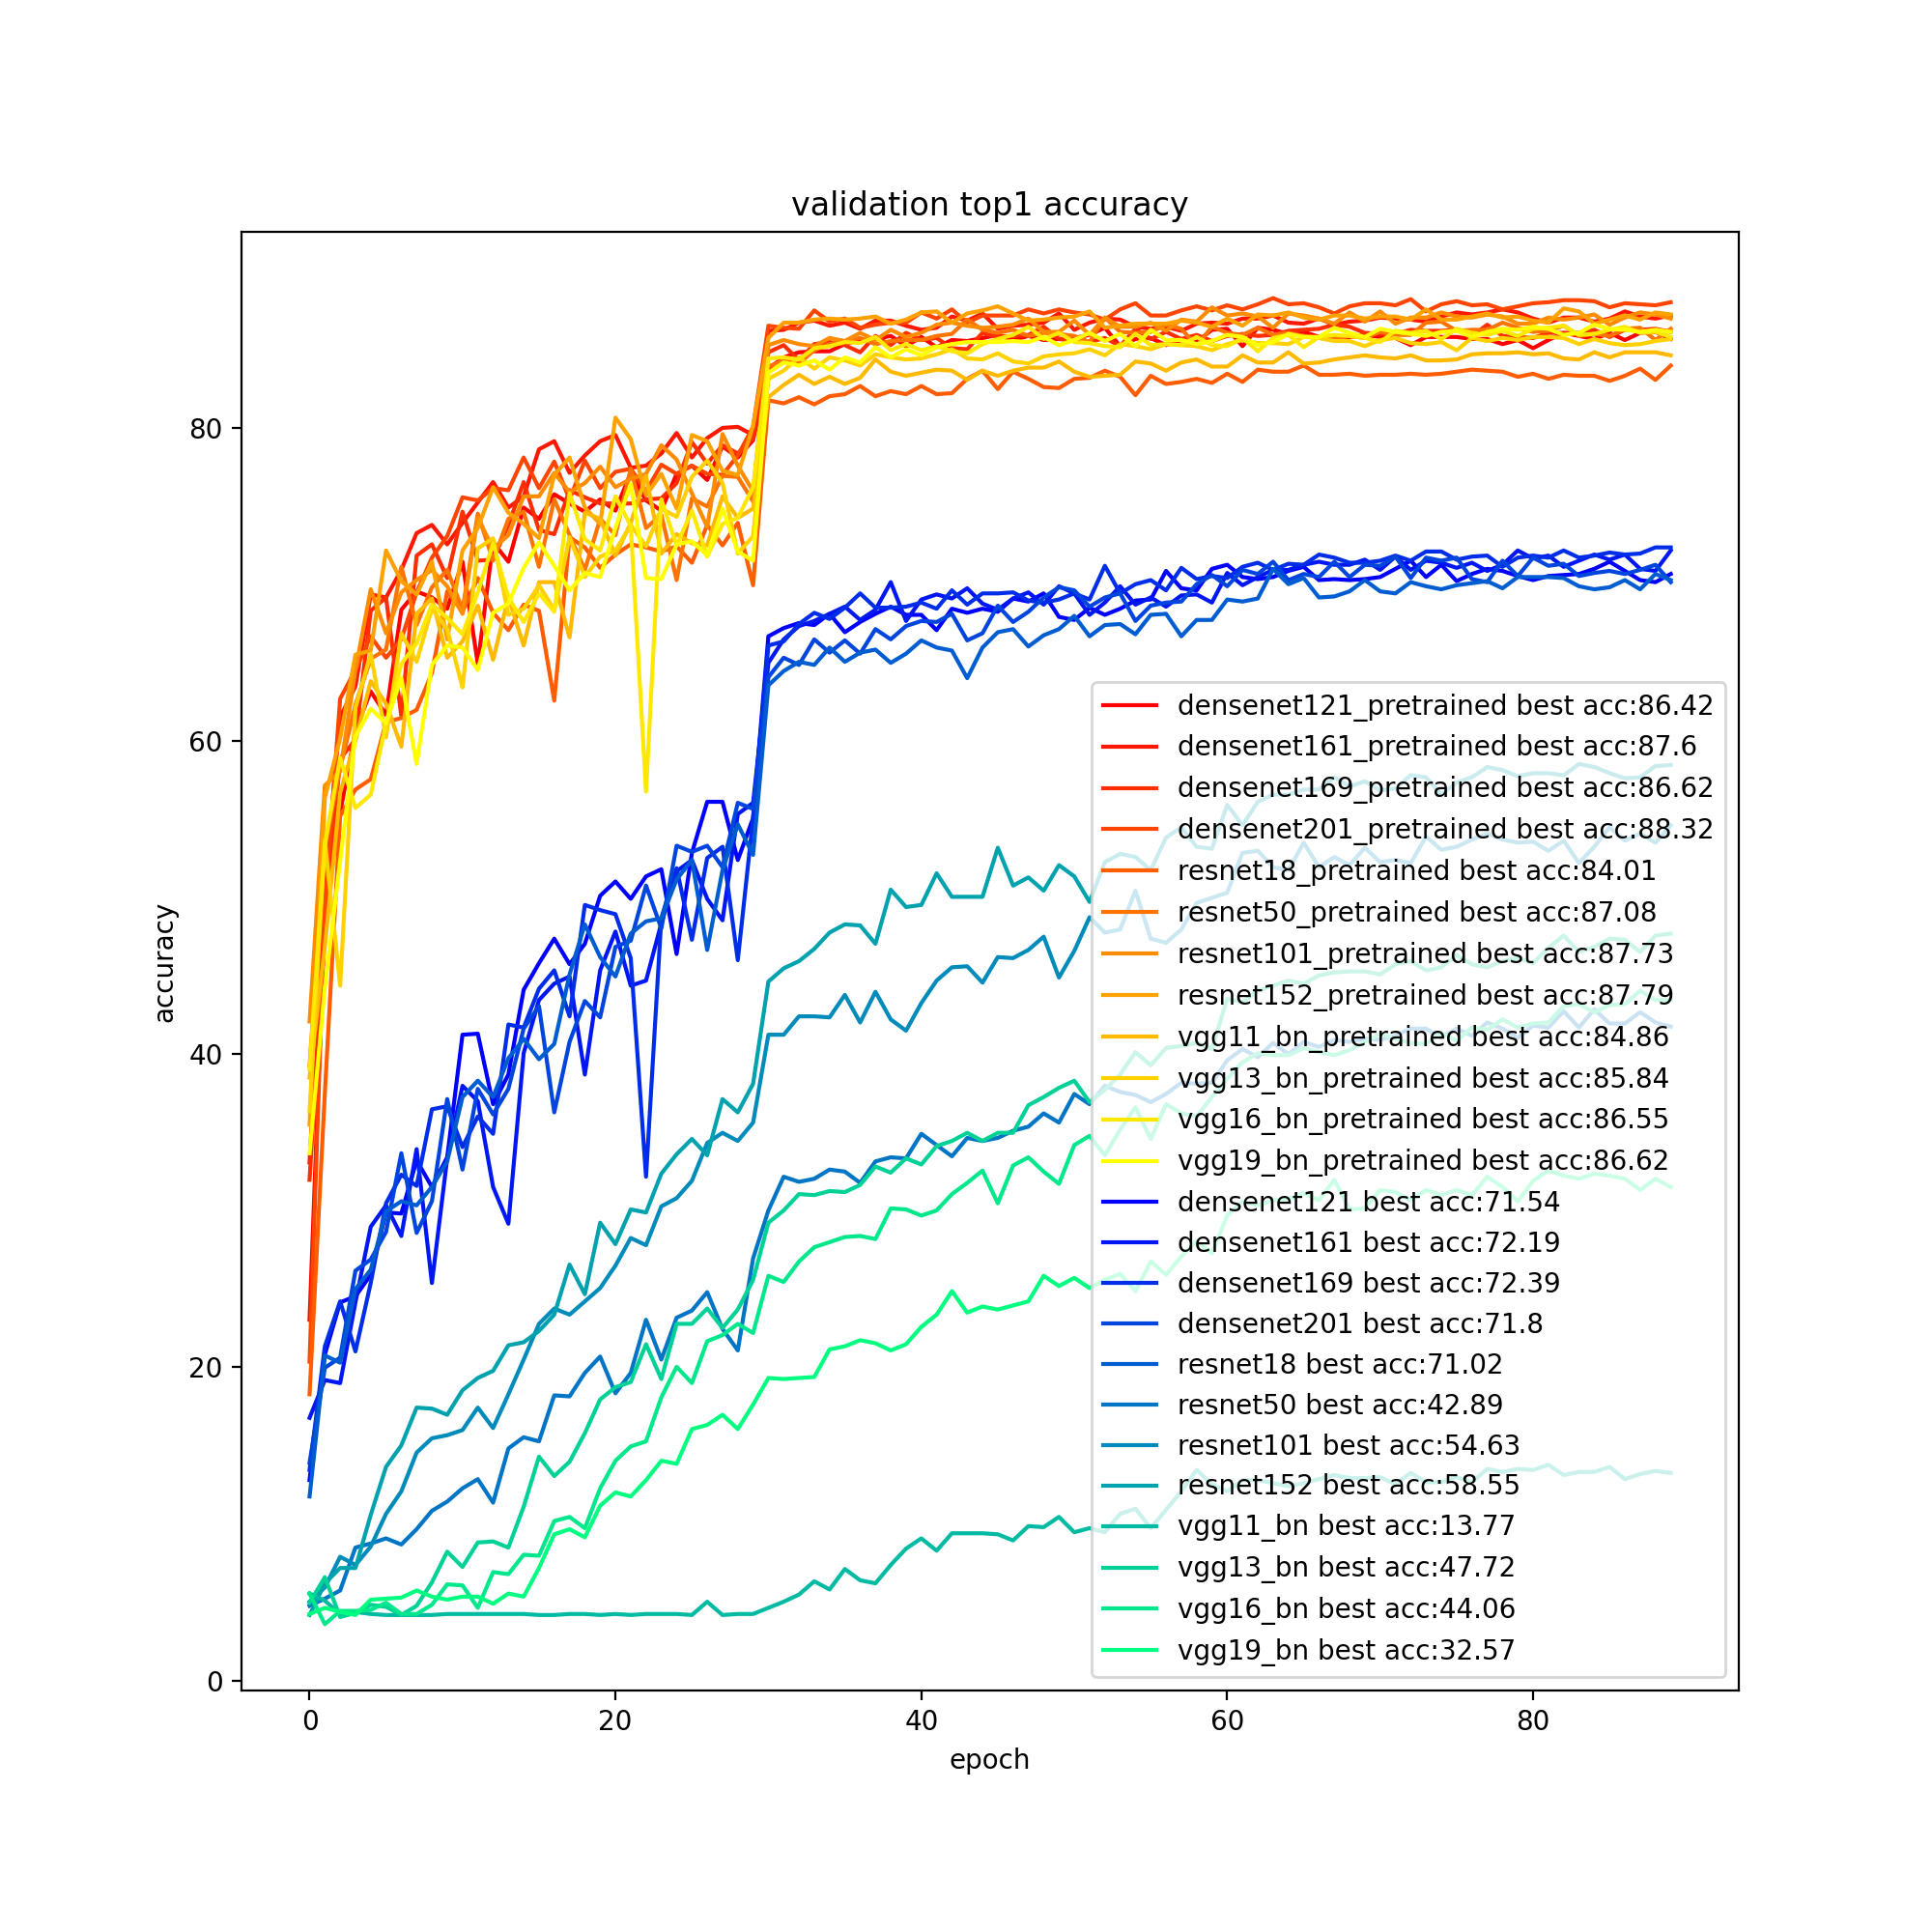
\includegraphics[scale=0.4]{figs/val_acc1.png}
%   \caption{Top-1 Validation Accuracy of Baseline Models}
%   \label{fig:val_acc1}
% \end{figure}

% \begin{figure}[ht]
%   \centering
%   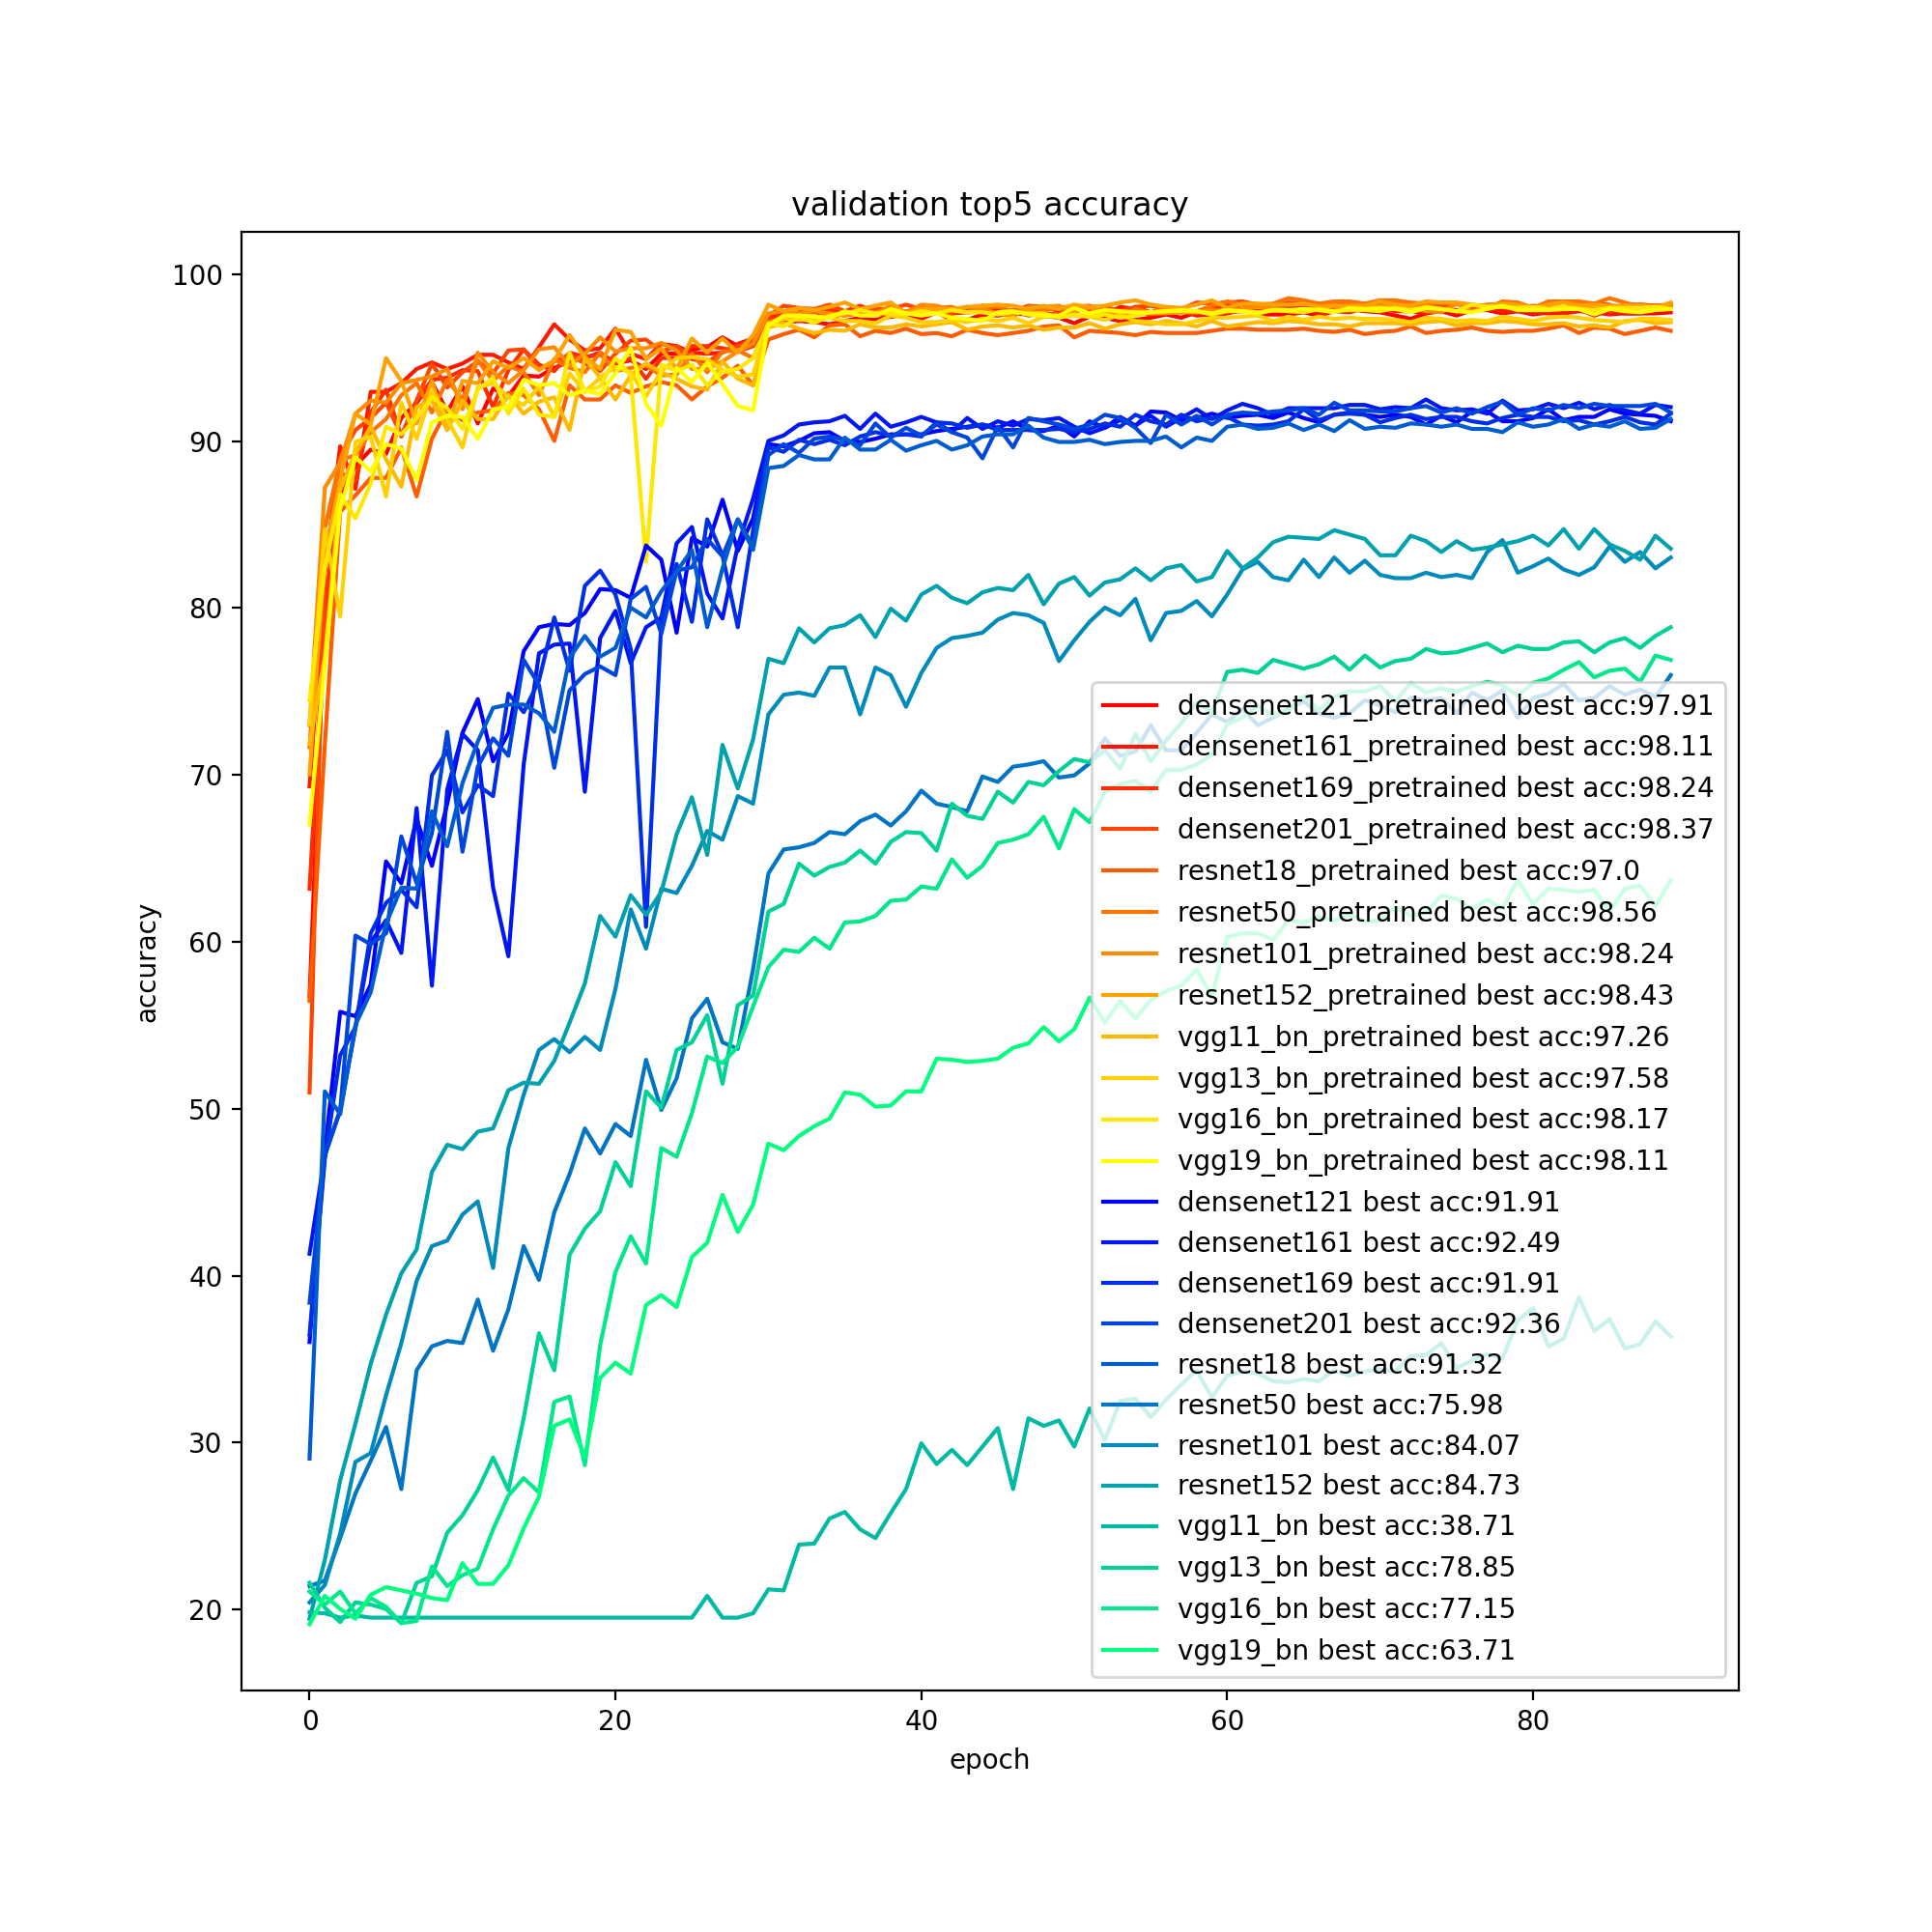
\includegraphics[scale=0.4]{figs/val_acc5.png}
%   \caption{Top-5 Validation Accuracy of Baseline Models}
%   \label{fig:val_acc5}
% \end{figure}

\begin{table}
  \centering
  \caption{Train Accuracy of Baseline Models}
  \label{tabel:train_acc}
  \begin{tabular}{ccc}
    \hline
    \toprule
    model                   & train top1 acc     & train top5 acc     \\
    \midrule  % 中部线
    densenet161\_pretrained & 96.9 & 99.6 \\
    resnet152\_pretrained   & 96.9 & 99.5 \\
    densenet201\_pretrained & 96.6 & 99.4 \\
    resnet101\_pretrained   & 96.5 & 99.5 \\
    densenet169\_pretrained & 96.0 & 99.3 \\
    resnet50\_pretrained    & 95.6 & 99.3 \\
    densenet121\_pretrained & 95.3 & 99.3 \\
    resnet18\_pretrained    & 94.3 & 99.0 \\
    vgg16\_bn\_pretrained   & 93.4 & 98.7 \\
    vgg13\_bn\_pretrained   & 93.4 & 98.8 \\
    vgg11\_bn\_pretrained   & 93.0 & 98.7 \\
    vgg19\_bn\_pretrained   & 93.0 & 98.6 \\
    densenet161             & 86.0 & 97.4 \\
    densenet201             & 84.6 & 97.0 \\
    densenet169             & 84.2 & 96.9 \\
    densenet121             & 83.8 & 96.9 \\
    resnet18                & 79.0 & 95.6 \\
    resnet152               & 63.7 & 89.1 \\
    resnet101               & 55.5 & 84.8 \\
    resnet50                & 41.6 & 73.9 \\
    vgg13\_bn               & 41.4 & 74.8 \\
    vgg16\_bn               & 38.6 & 72.4 \\
    vgg19\_bn               & 26.9 & 59.6 \\
    vgg11\_bn               & 11.8 & 34.3 \\
    \bottomrule
  \end{tabular}
\end{table}

\begin{table}
  \centering
  \caption{Validation Accuracy of Baseline Models}
  \label{tabel:val_acc}
  \begin{tabular}{ccc}
    \hline
    \toprule
    model                   & val top1 acc       & val top5 acc      \\
    \midrule  % 中部线

    densenet201\_pretrained & 88.3 & 98.4 \\
    resnet152\_pretrained   & 87.8 & 98.4 \\
    resnet101\_pretrained   & 87.7 & 98.2 \\
    densenet161\_pretrained & 87.6 & 98.1 \\
    resnet50\_pretrained    & 87.1 & 98.6 \\
    densenet169\_pretrained & 86.6 & 98.2 \\
    vgg19\_bn\_pretrained   & 86.6 & 98.1 \\
    vgg16\_bn\_pretrained   & 86.6 & 98.2 \\
    densenet121\_pretrained & 86.4 & 97.9 \\
    vgg13\_bn\_pretrained   & 85.8 & 97.6 \\
    vgg11\_bn\_pretrained   & 84.9 & 97.3 \\
    resnet18\_pretrained    & 84.0 & 97.0 \\
    densenet169             & 72.4 & 91.9 \\
    densenet161             & 72.2 & 92.5 \\
    densenet201             & 71.8 & 92.4 \\
    densenet121             & 71.5 & 91.9 \\
    resnet18                & 71.0 & 91.3 \\
    resnet152               & 58.6 & 84.7 \\
    resnet101               & 54.6 & 84.1 \\
    vgg13\_bn               & 47.7 & 78.9 \\
    vgg16\_bn               & 44.1 & 77.2 \\
    resnet50                & 42.9 & 76.0 \\
    vgg19\_bn               & 32.6 & 63.7 \\
    vgg11\_bn               & 13.8 & 38.7 \\
    \bottomrule
  \end{tabular}
\end{table}

\subsubsection{Confusion Matrix}
A Confusion matrix is an N x N matrix used for evaluating the performance of a classification model, where N is the number of target classes. The matrix compares the actual target values with those predicted by the machine learning model. This gives us a holistic view of how well our classification model is performing and what kinds of errors it is making\cite{conf_matrix}.

We draw the validation confusion matrix of all the models. To better observe the mismatched cases, we also add a log function to the matrix values, reducing the gap between maximum and minimum values. The results are shown from Figure \ref{fig:vgg11_conf} to Figure \ref{fig:densenet201_conf}.

\begin{figure}[t]
  \begin{minipage}[b]{.5\linewidth}
    \centering
    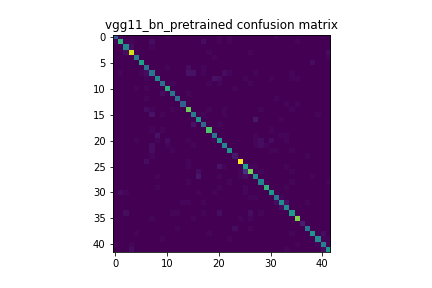
\includegraphics[width=1.2\textwidth]{figs/conf_matrix/vgg11_bn_pretrained_conf.png}
    \subcaption{Pretrained VGG11}
  \end{minipage}
  \hfill
  \begin{minipage}[b]{.5\linewidth}
    \centering
    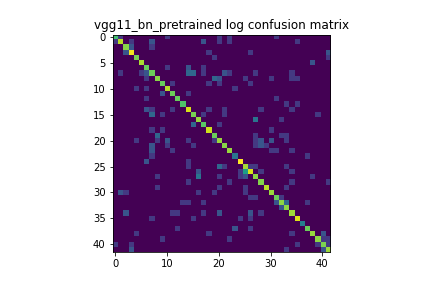
\includegraphics[width=1.2\textwidth]{figs/conf_matrix/vgg11_bn_pretrained_log_conf.png}
    \subcaption{Log Pretrained VGG11}
  \end{minipage}
  \vfill
  \begin{minipage}[b]{.5\linewidth}
    \centering
    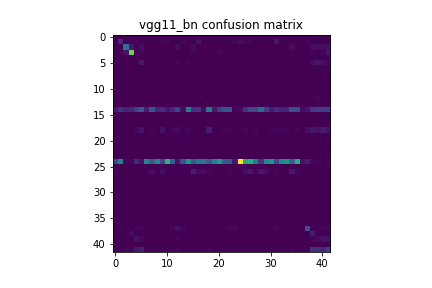
\includegraphics[width=1.2\textwidth]{figs/conf_matrix/vgg11_bn_conf.png}
    \subcaption{Non-pretrained VGG11}
  \end{minipage}
  \hfill
  \begin{minipage}[b]{.5\linewidth}
    \centering
    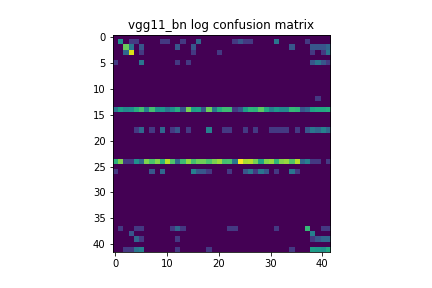
\includegraphics[width=1.2\textwidth]{figs/conf_matrix/vgg11_bn_log_conf.png}
    \subcaption{Log Non-pretrained VGG11}
  \end{minipage}
  \caption{Confusion Matrix of VGG11}
  \label{fig:vgg11_conf}
\end{figure}

\begin{figure}[t]

  \begin{minipage}[t]{.5\linewidth}
    \centering
    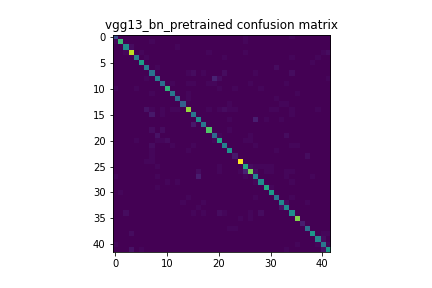
\includegraphics[width=1.2\textwidth]{figs/conf_matrix/vgg13_bn_pretrained_conf.png}
    \subcaption{Pretrained VGG13}
  \end{minipage}
  \hfill
  \begin{minipage}[t]{.5\linewidth}
    \centering
    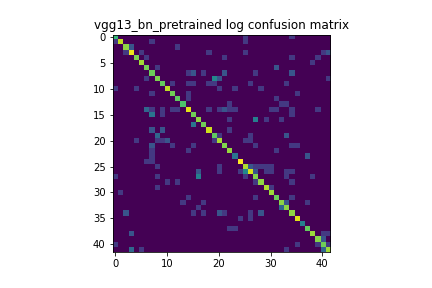
\includegraphics[width=1.2\textwidth]{figs/conf_matrix/vgg13_bn_pretrained_log_conf.png}
    \subcaption{Log Pretrained VGG13}
  \end{minipage}
  \vfill
  \begin{minipage}[b]{.5\linewidth}
    \centering
    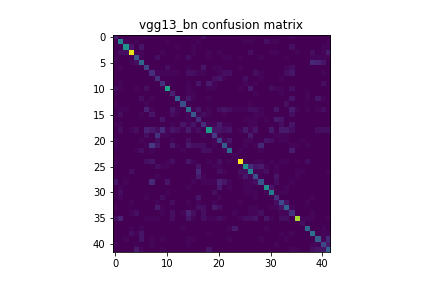
\includegraphics[width=1.2\textwidth]{figs/conf_matrix/vgg13_bn_conf.png}
    \subcaption{Non-pretrained VGG13}
  \end{minipage}
  \hfill
  \begin{minipage}[b]{.5\linewidth}
    \centering
    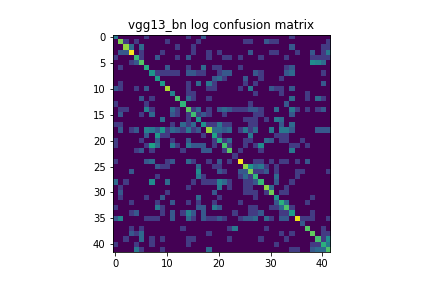
\includegraphics[width=1.2\textwidth]{figs/conf_matrix/vgg13_bn_log_conf.png}
    \subcaption{Log Non-pretrained VGG13}
  \end{minipage}

  \caption{Confusion Matrix of VGG13}
  \vspace{-3mm}
  \label{fig:vgg13_conf}
\end{figure}

\begin{figure}[t]
  \begin{minipage}[b]{.5\linewidth}
    \centering
    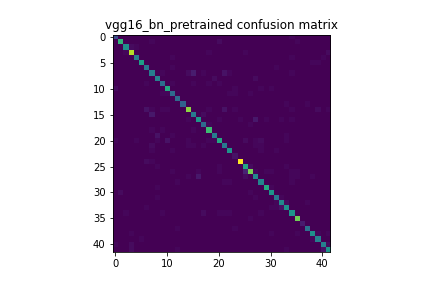
\includegraphics[width=1.2\textwidth]{figs/conf_matrix/vgg16_bn_pretrained_conf.png}
    \subcaption{Pretrained VGG16}
  \end{minipage}
  \hfill
  \begin{minipage}[b]{.5\linewidth}
    \centering
    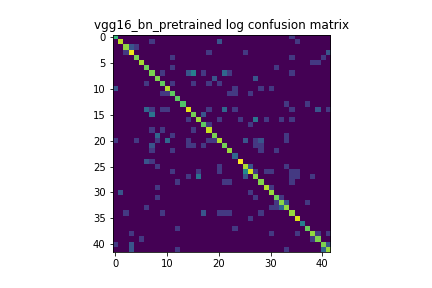
\includegraphics[width=1.2\textwidth]{figs/conf_matrix/vgg16_bn_pretrained_log_conf.png}
    \subcaption{Log Pretrained VGG16}
  \end{minipage}
  \vfill
  \begin{minipage}[b]{.5\linewidth}
    \centering
    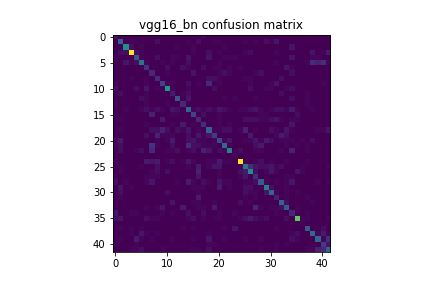
\includegraphics[width=1.2\textwidth]{figs/conf_matrix/vgg16_bn_conf.png}
    \subcaption{Non-pretrained VGG16}
  \end{minipage}
  \hfill
  \begin{minipage}[b]{.5\linewidth}
    \centering
    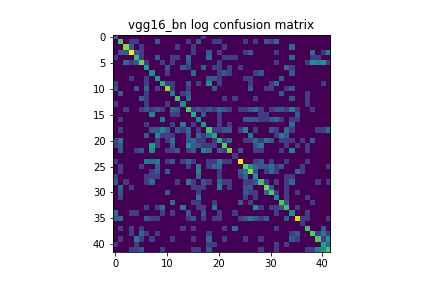
\includegraphics[width=1.2\textwidth]{figs/conf_matrix/vgg16_bn_log_conf.png}
    \subcaption{Log Non-pretrained VGG16}
  \end{minipage}

  \caption{Confusion Matrix of VGG16}
  \label{fig:vgg16_conf}
\end{figure}

\begin{figure}[t]

  \begin{minipage}[b]{.5\linewidth}
    \centering
    {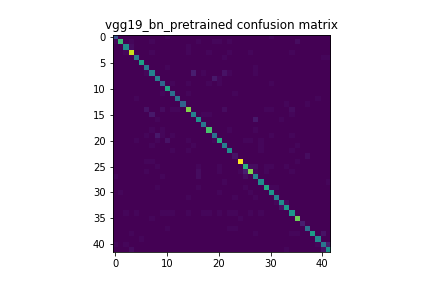
\includegraphics[width=1.2\textwidth]{figs/conf_matrix/vgg19_bn_pretrained_conf.png}}
    \subcaption{Pretrained VGG19}
  \end{minipage}
  \hfill
  \begin{minipage}[b]{.5\linewidth}
    \centering
    {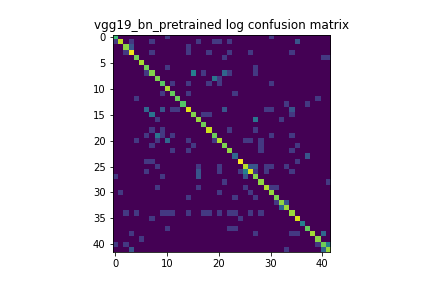
\includegraphics[width=1.2\textwidth]{figs/conf_matrix/vgg19_bn_pretrained_log_conf.png}}
    \subcaption{Log Pretrained VGG19}
  \end{minipage}
  \vfill
  \begin{minipage}[b]{.5\linewidth}
    \centering
    {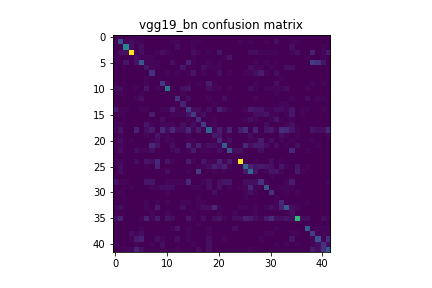
\includegraphics[width=1.2\textwidth]{figs/conf_matrix/vgg19_bn_conf.png}}
    \subcaption{Non-pretrained VGG19}
  \end{minipage}
  \hfill
  \begin{minipage}[b]{.5\linewidth}
    \centering
    {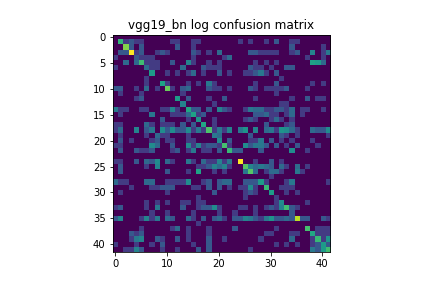
\includegraphics[width=1.2\textwidth]{figs/conf_matrix/vgg19_bn_log_conf.png}}
    \subcaption{Log Non-pretrained VGG19}
  \end{minipage}

  \caption{Confusion Matrix of VGG19}
  \label{fig:vgg19_conf}
  \vspace{0.2in}
\end{figure}

\begin{figure}[t]
  \begin{minipage}[b]{.5\linewidth}
    \centering
    {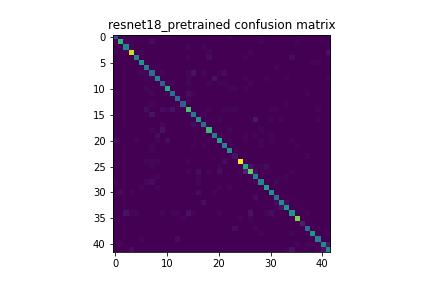
\includegraphics[width=1.2\textwidth]{figs/conf_matrix/resnet18_pretrained_conf.png}}
    \subcaption{Pretrained ResNet18}
  \end{minipage}
  \hfill
  \begin{minipage}[b]{.5\linewidth}
    \centering
    {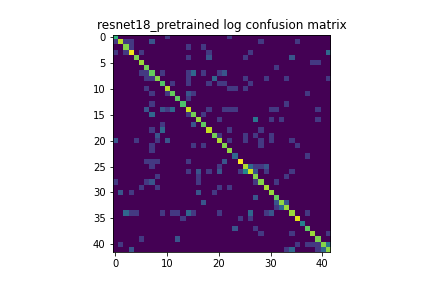
\includegraphics[width=1.2\textwidth]{figs/conf_matrix/resnet18_pretrained_log_conf.png}}
    \subcaption{Log Pretrained ResNet18}
  \end{minipage}
  \vfill
  \begin{minipage}[b]{.5\linewidth}
    \centering
    {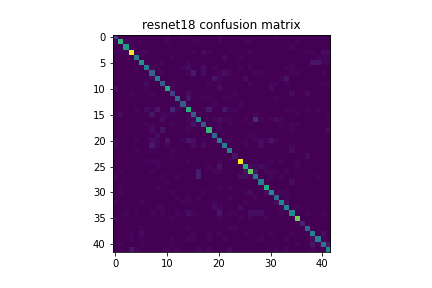
\includegraphics[width=1.2\textwidth]{figs/conf_matrix/resnet18_conf.png}}
    \subcaption{Non-pretrained ResNet18}
  \end{minipage}
  \hfill
  \begin{minipage}[b]{.5\linewidth}
    \centering

    {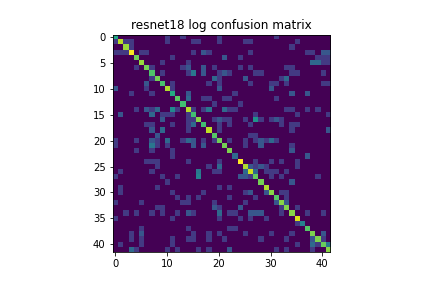
\includegraphics[width=1.2\textwidth]{figs/conf_matrix/resnet18_log_conf.png}}
    \subcaption{Log Non-pretrained ResNet18}
  \end{minipage}

  \caption{Confusion Matrix of ResNet18}
  \label{fig:resnet18_conf}
  \vspace{0.2in}
\end{figure}

\begin{figure}[t]
  \begin{minipage}[b]{.5\linewidth}
    \centering
    {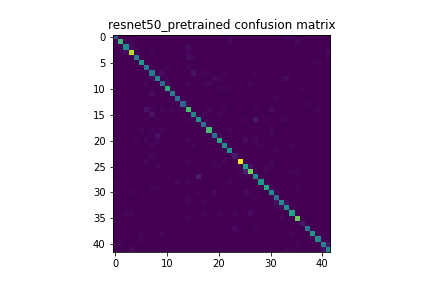
\includegraphics[width=1.2\textwidth]{figs/conf_matrix/resnet50_pretrained_conf.png}}
    \subcaption{Pretrained ResNet50}
  \end{minipage}
  \hfill
  \begin{minipage}[b]{.5\linewidth}
    \centering

    {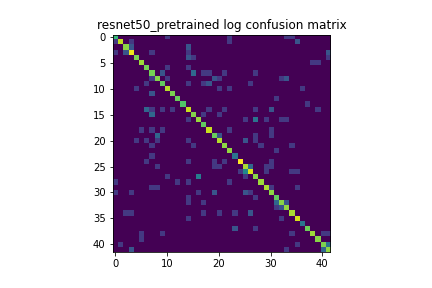
\includegraphics[width=1.2\textwidth]{figs/conf_matrix/resnet50_pretrained_log_conf.png}}
    \subcaption{Log Pretrained ResNet50}
  \end{minipage}
  \vfill
  \begin{minipage}[b]{.5\linewidth}
    \centering

    {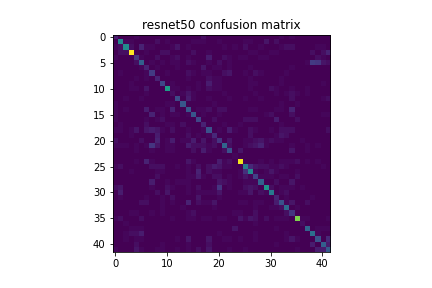
\includegraphics[width=1.2\textwidth]{figs/conf_matrix/resnet50_conf.png}}
    \subcaption{Non-pretrained ResNet50}
  \end{minipage}
  \hfill
  \begin{minipage}[b]{.5\linewidth}
    \centering

    {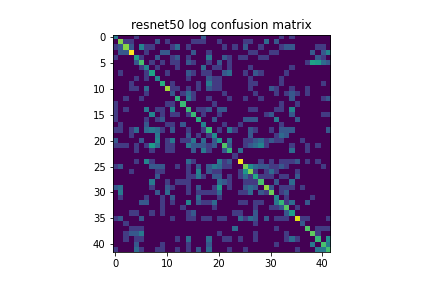
\includegraphics[width=1.2\textwidth]{figs/conf_matrix/resnet50_log_conf.png}}
    \subcaption{Log Non-pretrained ResNet50}
  \end{minipage}

  \caption{Confusion Matrix of ResNet50}
  \label{fig:resnet50_conf}
  \vspace{0.2in}
\end{figure}

\begin{figure}[t]
  \begin{minipage}[b]{.5\linewidth}
    \centering
    {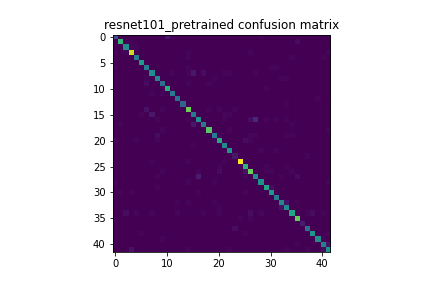
\includegraphics[width=1.2\textwidth]{figs/conf_matrix/resnet101_pretrained_conf.png}}
    \subcaption{Pretrained ResNet101}
  \end{minipage}
  \hfill
  \begin{minipage}[b]{.5\linewidth}
    \centering

    {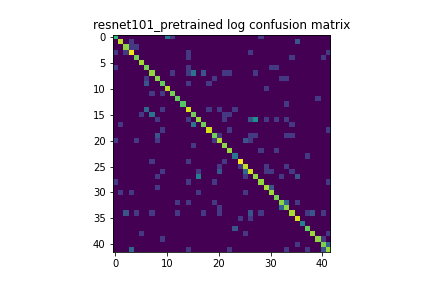
\includegraphics[width=1.2\textwidth]{figs/conf_matrix/resnet101_pretrained_log_conf.png}}
    \subcaption{Log Pretrained ResNet101}
  \end{minipage}
  \vfill
  \begin{minipage}[b]{.5\linewidth}
    \centering

    {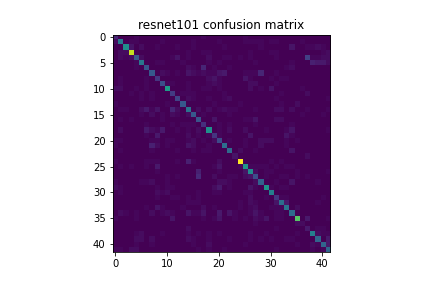
\includegraphics[width=1.2\textwidth]{figs/conf_matrix/resnet101_conf.png}}
    \subcaption{Non-pretrained ResNet101}
  \end{minipage}
  \hfill
  \begin{minipage}[b]{.5\linewidth}
    \centering

    {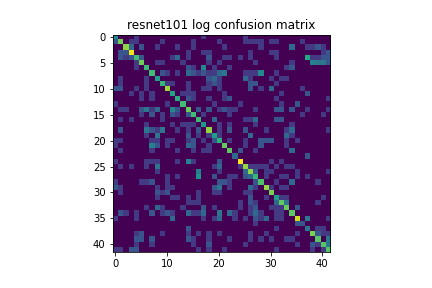
\includegraphics[width=1.2\textwidth]{figs/conf_matrix/resnet101_log_conf.png}}
    \subcaption{Log Non-pretrained ResNet101}

  \end{minipage}

  \caption{Confusion Matrix of ResNet101}
  \label{fig:resnet101_conf}
  \vspace{0.2in}
\end{figure}

\begin{figure}[t]
  \begin{minipage}[b]{.5\linewidth}
    \centering
    {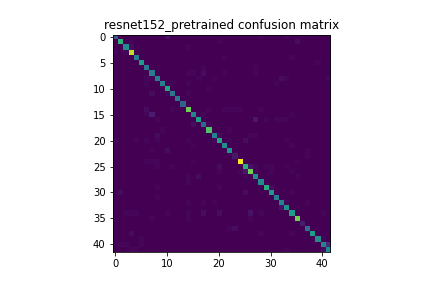
\includegraphics[width=1.2\textwidth]{figs/conf_matrix/resnet152_pretrained_conf.png}}
    \subcaption{Pretrained ResNet152}
  \end{minipage}
  \hfill
  \begin{minipage}[b]{.5\linewidth}
    \centering

    {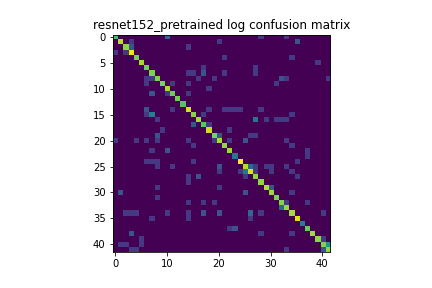
\includegraphics[width=1.2\textwidth]{figs/conf_matrix/resnet152_pretrained_log_conf.png}}
    \subcaption{Log Pretrained ResNet152}
  \end{minipage}
  \vfill
  \begin{minipage}[b]{.5\linewidth}
    \centering

    {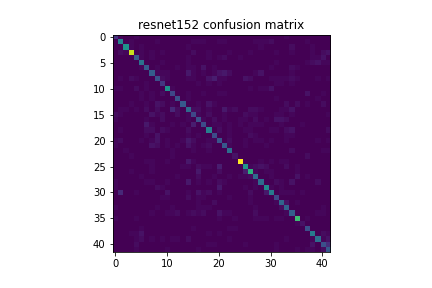
\includegraphics[width=1.2\textwidth]{figs/conf_matrix/resnet152_conf.png}}
    \subcaption{Non-pretrained ResNet152}
  \end{minipage}
  \hfill
  \begin{minipage}[b]{.5\linewidth}
    \centering

    {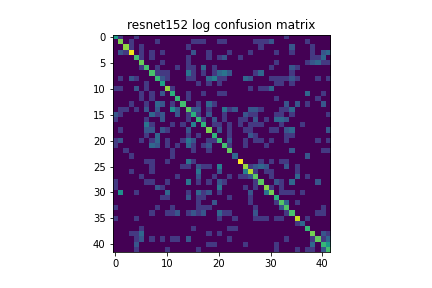
\includegraphics[width=1.2\textwidth]{figs/conf_matrix/resnet152_log_conf.png}}
    \subcaption{Log Non-pretrained ResNet152}
  \end{minipage}

  \caption{Confusion Matrix of ResNet152}
  \label{fig:resnet152_conf}
  \vspace{0.2in}
\end{figure}

\begin{figure}[t]
  \begin{minipage}[b]{.5\linewidth}
    \centering
    {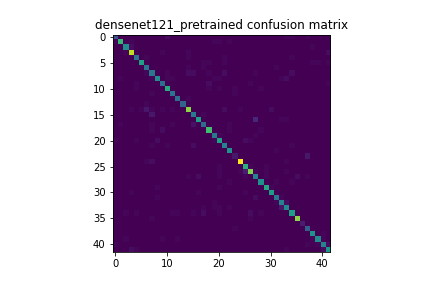
\includegraphics[width=1.2\textwidth]{figs/conf_matrix/densenet121_pretrained_conf.png}}
    \subcaption{Pretrained DenseNet121}
  \end{minipage}
  \hfill
  \begin{minipage}[b]{.5\linewidth}
    \centering

    {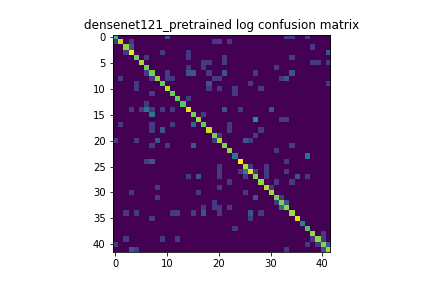
\includegraphics[width=1.2\textwidth]{figs/conf_matrix/densenet121_pretrained_log_conf.png}}
    \subcaption{Log Pretrained DenseNet121}
  \end{minipage}
  \vfill
  \begin{minipage}[b]{.5\linewidth}
    \centering

    {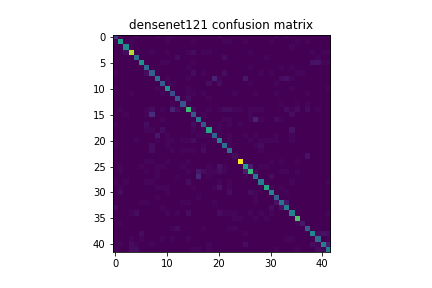
\includegraphics[width=1.2\textwidth]{figs/conf_matrix/densenet121_conf.png}}
    \subcaption{Non-pretrained DenseNet121}
  \end{minipage}
  \hfill
  \begin{minipage}[b]{.5\linewidth}
    \centering

    {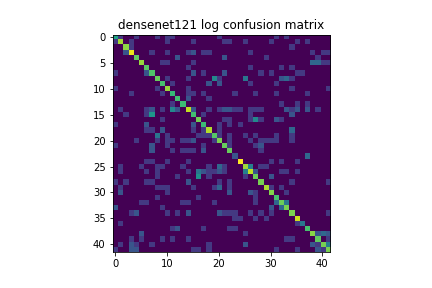
\includegraphics[width=1.2\textwidth]{figs/conf_matrix/densenet121_log_conf.png}}
    \subcaption{Log Non-pretrained DenseNet121}

  \end{minipage}

  \caption{Confusion Matrix of DenseNet121}
  \label{fig:densenet121_conf}
  \vspace{0.2in}
\end{figure}

\begin{figure}[t]
  \begin{minipage}[b]{.5\linewidth}
    \centering
    {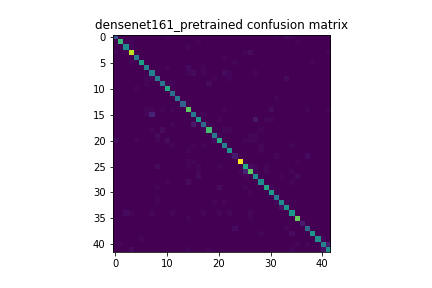
\includegraphics[width=1.2\textwidth]{figs/conf_matrix/densenet161_pretrained_conf.png}}
    \subcaption{Pretrained DenseNet161}
  \end{minipage}
  \hfill
  \begin{minipage}[b]{.5\linewidth}
    \centering

    {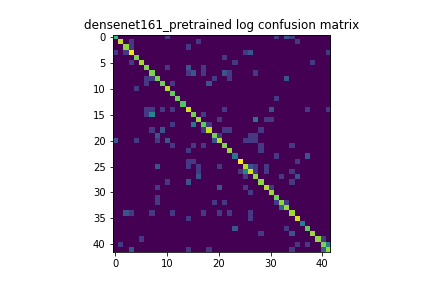
\includegraphics[width=1.2\textwidth]{figs/conf_matrix/densenet161_pretrained_log_conf.png}}
    \subcaption{Log Pretrained DenseNet161}
  \end{minipage}
  \vfill
  \begin{minipage}[b]{.5\linewidth}
    \centering

    {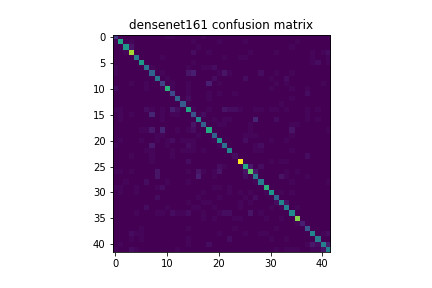
\includegraphics[width=1.2\textwidth]{figs/conf_matrix/densenet161_conf.png}}
    \subcaption{Non-pretrained DenseNet161}
  \end{minipage}
  \hfill
  \begin{minipage}[b]{.5\linewidth}
    \centering

    {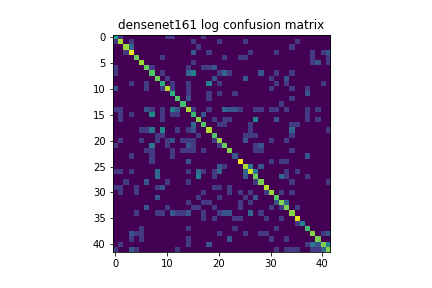
\includegraphics[width=1.2\textwidth]{figs/conf_matrix/densenet161_log_conf.png}}
    \subcaption{Log Non-pretrained DenseNet161}
  \end{minipage}

  \caption{Confusion Matrix of DenseNet161}
  \label{fig:densenet161_conf}
  \vspace{0.2in}
\end{figure}

\begin{figure}[t]
  \begin{minipage}[b]{.5\linewidth}
    \centering
    {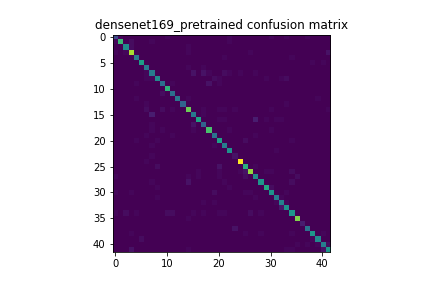
\includegraphics[width=1.2\textwidth]{figs/conf_matrix/densenet169_pretrained_conf.png}}
    \subcaption{Pretrained DenseNet169}
  \end{minipage}
  \hfill
  \begin{minipage}[b]{.5\linewidth}
    \centering

    {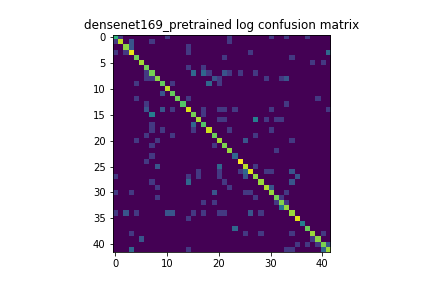
\includegraphics[width=1.2\textwidth]{figs/conf_matrix/densenet169_pretrained_log_conf.png}}
    \subcaption{Log Pretrained DenseNet169}
  \end{minipage}
  \vfill
  \begin{minipage}[b]{.5\linewidth}
    \centering

    {\includegraphics[width=1.2\textwidth]{figs/conf_matrix/densenet169_conf.png}}
    \subcaption{Non-pretrained DenseNet169}
  \end{minipage}
  \hfill
  \begin{minipage}[b]{.5\linewidth}
    \centering

    {\includegraphics[width=1.2\textwidth]{figs/conf_matrix/densenet169_log_conf.png}}
    \subcaption{Log Non-pretrained DenseNet169}
  \end{minipage}

  \caption{Confusion Matrix of DenseNet169}
  \label{fig:densenet169_conf}
  \vspace{0.2in}
\end{figure}

\begin{figure}[t]
  \begin{minipage}[b]{.5\linewidth}
    \centering
    {\includegraphics[width=1.2\textwidth]{figs/conf_matrix/densenet201_pretrained_conf.png}}
    \subcaption{Pretrained DenseNet201}
  \end{minipage}
  \hfill
  \begin{minipage}[b]{.5\linewidth}
    \centering

    {\includegraphics[width=1.2\textwidth]{figs/conf_matrix/densenet201_pretrained_log_conf.png}}
    \subcaption{Log Pretrained DenseNet201}
  \end{minipage}
  \vfill
  \begin{minipage}[b]{.5\linewidth}
    \centering

    {\includegraphics[width=1.2\textwidth]{figs/conf_matrix/densenet201_conf.png}}
    \subcaption{Non-pretrained DenseNet201}
  \end{minipage}
  \hfill
  \begin{minipage}[b]{.5\linewidth}
    \centering

    {\includegraphics[width=1.2\textwidth]{figs/conf_matrix/densenet201_log_conf.png}}
    \subcaption{Log Non-pretrained DenseNet201}
  \end{minipage}


  \caption{Confusion Matrix of DenseNet201}
  \label{fig:densenet201_conf}
  \vspace{0.2in}
\end{figure}

\subsubsection{Precision, Recall and F1-score}
The model prediction can be classified into four cases: true positive (TP), true negative (TN), false positive (FP), and false negative(FN). After counting the number of these four cases, the computation of precision and recall is as following equations:


\begin{equation*}
  \begin{split}
    Precision & = \frac{TP}{TP+FP}\\
    Recall & = \frac{TP}{TP+FN}\\
  \end{split}
\end{equation*}

Considering a disease diagnosis scenario, precision is the measure of patients that the model correctly identify having a disease out of all the patients actually having it. Recall is how many we correctly identified as having a disease. Precision and recall are often in tension. That is, improving precision typically reduces recall. We need to balance the precision-recall tradeoff in real-world application.

F1-score is computed using the value of precision and recall:


\begin{equation*}
  \begin{split}
    F1 =2\times \frac{Precision  *Recall}{Precision + Recall}\\
  \end{split}
\end{equation*}

F1-score can be seen as a balance between precision and recall. Compared to accuracy, F1-score can better evaluate model generalization performance when the data distribution is unbalanced.

\subsection{Baseline Summary}
We compute all of the metrics on all the models, and concluded as Table \ref{tabel:f1}. We also rank the model based on different evaluation metrics, as shown in Figure \ref{fig:rank}. From multi-dimensional results, we observed that models with identical shortcuts achives higher accuracy and F1-score than models without that. All of the pretrained models outperforms non-pretrained models at all the evaluation metrics, which have already built good generalization on the large ImageNet dataset. The accuracy gap between pretrained and non-pretrained models in VGGNet is lager than that in DenseNet and ResNet, indicating a harder training process in models without identical shortcut. Deeper networks often achieve better performance, indicating a powerful representation capacity.

Among all of 24 models, the pretrained DenseNet201 take the first place in both top1 validation accuracy and F1-score. The highest top1 validation accuracy is under 90\%, which means there is still large space for us to improve the model performance.

\begin{table}[t]
  \centering
  \caption{Precison, Recall and F1-score of Baseline Models}
  \label{tabel:f1}
  % \resizebox{\textwidth}{!}{
  \begin{tabular}{cccc}
    \hline
    \toprule
    model                   & precision & recall & f1score \\
    \midrule  % 中部线


    densenet201\_pretrained & 0.875     & 0.885  & 0.879   \\
    resnet152\_pretrained   & 0.877     & 0.882  & 0.877   \\
    resnet101\_pretrained   & 0.872     & 0.880  & 0.875   \\
    densenet161\_pretrained & 0.872     & 0.875  & 0.873   \\
    resnet50\_pretrained    & 0.864     & 0.874  & 0.867   \\
    vgg16\_bn\_pretrained   & 0.856     & 0.876  & 0.862   \\
    vgg19\_bn\_pretrained   & 0.858     & 0.868  & 0.861   \\
    densenet169\_pretrained & 0.857     & 0.866  & 0.859   \\
    densenet121\_pretrained & 0.857     & 0.861  & 0.858   \\
    vgg13\_bn\_pretrained   & 0.852     & 0.857  & 0.853   \\
    vgg11\_bn\_pretrained   & 0.846     & 0.848  & 0.846   \\
    resnet18\_pretrained    & 0.832     & 0.848  & 0.837   \\
    densenet169             & 0.712     & 0.733  & 0.718   \\
    densenet161             & 0.708     & 0.716  & 0.709   \\
    densenet201             & 0.706     & 0.713  & 0.706   \\
    resnet18                & 0.701     & 0.711  & 0.703   \\
    densenet121             & 0.696     & 0.710  & 0.700   \\
    resnet152               & 0.570     & 0.589  & 0.573   \\
    resnet101               & 0.523     & 0.534  & 0.520   \\
    vgg13\_bn               & 0.450     & 0.500  & 0.454   \\
    vgg16\_bn               & 0.409     & 0.463  & 0.406   \\
    resnet50                & 0.406     & 0.430  & 0.401   \\
    vgg19\_bn               & 0.286     & 0.288  & 0.270   \\
    vgg11\_bn               & 0.103     & 0.091  & 0.078   \\
    \bottomrule
  \end{tabular}
\end{table}

\begin{figure}[ht]
  \centering
  \includegraphics[width=\linewidth]{figs/rank.png}
  \caption{Performance Rank of Different Evaluation Metrics}
  \label{fig:rank}
\end{figure}

\subsection{Visualization of the activation feature map}
The activation function ReLU is defined as
\begin{equation}
  \text{ReLU}(x)=\left\{
  \begin{array}{lr}
    x, & x > 0    \\
    0, & x \leq 0
  \end{array}
  \right.
\end{equation}
We can condiser the ReLU activation function as a filter of features, thus the positive element means more important part.
By ploting the output of ReLU layer, we can visualize how the model processes the input images.
Due to the output features map of latter layers are too small to view, we only draw the output of the first ReLU layer.


As the Fig.~\ref{fig:actmap} shows, the model catch the knapsack in the image even though it is not on the center, showing the ability to 
extract features out of a images.

\begin{figure}[h]
  \begin{minipage}[b]{\linewidth}
    \centering
    \includegraphics[height=4cm]{figs/img_7224.jpg}
    \centerline{(a) The original paper}
    \vspace{1mm}
  \end{minipage}
  \begin{minipage}[b]{\linewidth}
    \centering
    \includegraphics[width=12cm]{figs/ReLU_2.jpg}
    \centerline{(b) The feature map of the first activation layer.}
  \end{minipage}
  \caption{Visualization of the activation map.}
  \label{fig:actmap}
\end{figure}